\chapter{Univalent Functions}\label{part3}

\setcounter{section}{3}
\setcounter{subsection}{0}
\subsection{Schlicht functions}\label{part3-sec3.1}\pageoriginale

\begin{defi*}
A function $f(z)$ regular in a domain $D$ is said to be {\em
  univalent} (Schlicht, Simple) if $f(z)$ takes different values at
different points of $D$. Then $f(z)$ maps $D$, one-one conformally
into a domain $\Delta$.
\end{defi*}

Since $f(z)$ takes no value more than once, if $f(z)$ is Schlicht in
the plane, the function $A(r)$ (area on the Riemann sphere) is less or
equal to one and $T_{0}(r)\leq \log r$. So $f(z)$ is rational and is
in fact a polynomial which must be linear. We consider functions
$f(z)$ univalent in $|z|<1$. If
$f(z)=\sum\limits^{\infty}_{n=0}a_{n}z^{n}$, $(f(z)-a_{0})/a_{1}$ is
also univalent. In fact $a_{1}$ cannot be zero, for otherwise $f(z)$
would assume values at least twice near $z=0$, $a_{1}\neq 0$. Hence we
may assume $f(z)$ to be of the form 
\begin{equation*}
z+\sum\limits^{\infty}_{n=2}a_{n}z^{n}\tag{2}\label{part3-eq2}
\end{equation*}
The class of functions, univalent in $|z|<1$ with the expansion
\eqref{part3-eq2} is called $S$.

The first two results are,

\setcounter{thm}{0}
\begin{thm}\label{part3-thm1}
If $f(z)\in S$, $|a_{2}|\leq 2$, and equality is possible only for
$f(z)=f_{\theta}(z)=\dfrac{z}{[1-ze^{i\theta}]^{2}}$, and
\end{thm}

\begin{thm}\label{part3-thm2}
If $f(z)\in S$ and $w$ is a value not taken by $f(z)$ then $|w|\geq
\frac{1}{4}$, again equality is possible only for
$f(z)=f_{\theta}(z)$. 
\end{thm}

Both\pageoriginale results in the above form are due to Biberbach,
theorem \ref{part3-thm2} with a smaller constant than $\frac{1}{4}$ is
due to Koebe though it seems we had the proof eventually form

Note that $f(z)\in S$, takes all values with modulus
$<\frac{1}{4}$. We shall prove theorem \ref{part3-thm1} first and then
deduce theorem \ref{part3-thm2} from it. For that we need

\setcounter{lem}{0}
\begin{lem}\label{part3-lem1}
Suppose $f(z)$ is regular and univalent in the annulus
$r_{1}<|z|<r_{2}$ then the area of the image of the annulus is
$\pi\sum\limits^{\infty}_{-\infty}n|a_{n}|^{2}(r^{2n}_{2}-r^{2n}_{1})$,
where $f(z)$ has the expansion
$\sum\limits^{\infty}_{-\infty}a_{n}z^{n}$ in the annulus.
\end{lem}

\begin{proof}
The area of the image is clearly $\int\limits^{r_{2}}_{r_{1}}r\ dr
\int\limits^{2\pi}_{0}|f'(re^{i\theta})|^{2}d\theta$. The integral
\begin{align*}
\int\limits^{2\pi}_{0}|f'(re^{i\theta})|^{2}d\theta &=
\int\limits^{2\pi}_{0}f'(re^{i\theta})\ob{f(re^{i\theta})}d\theta\\
&=\int\limits^{2\pi}_{0}\left[\sum
  na_{n}r^{n-1}e^{i(n-1)\theta}\right]\left[\sum
  m\ob{a}_{m}r^{m-1}e^{-i(m-1)\theta}\right]   
\end{align*}
Since the multiplication of the two series and then term by term
integrations are valid, and
$
\int\limits^{2\pi}_{0}e^{i(m-n)\theta}d\theta= \begin{cases}
0, & m\neq n,\\
2\pi,& m=n.
\end{cases}
$
$$
\int\limits^{2\pi}_{0}|f'(re^{i\theta})|^{2}d\theta=2\pi\sum^{\infty}_{-\infty}n^{2}|a_{n}|^{2}r^{2n-2}
$$
$\therefore$\pageoriginale Area of image
\begin{align*}
&=
  \int\limits^{r_{2}}_{r_{1}}r\ dr\int\limits^{2\pi}_{0}|f(re^{i\theta})|^{2}d\theta\\
&= 2\pi \int\limits^{r_{2}}_{r_{1}}\sum^{+\infty}_{-\infty}n^{2}|a_{n}|^{2}r^{2n-1}dt.
\end{align*}
Again since integration term by term is valid,
$$
=\pi\sum^{+\infty}_{-\infty}n|a_{n}|^{2}(r^{2n}_{2}-r^{2n}_{1})
$$
Hence the lemma.
\end{proof}

We now proceed to prove the theorem.

Consider the function $f(z)\in S$.
\begin{align*}
f(z)=z+\sum^{\infty}_{2}a_{n}z^{n},\quad\text{let}\quad F(z) &=
\left[f(z^{2})\right]^{\frac{1}{2}}=z\left[\frac{f(z^{2})}{z^{2}}\right]^{\frac{1}{2}}\\
&= z\left[1+\sum^{\infty}_{2}a_{n}z^{2n-2}\right]^{\frac{1}{2}}
\end{align*}
Since $\dfrac{f(z)}{z}$ is not zero $\dfrac{f(z)}{z}$ has a one valued
square root which is a power series in $z$ and hence
$\left[\dfrac{f(z^{2})}{z^{2}}\right]^{\frac{1}{2}}$ is a power series
in $z^{2}$.
$$
F(z)=z+\frac{1}{2}a_{2}z^{3}+\cdots\cdots
$$
$F(z)$ is odd. Also $F(z)$ is univalent. For if $F(z_{1})=F(z_{2})$,
then 
$$
\left[f(z^{2}_{1})\right]^{\frac{1}{2}}=\left[f(z^{2}_{2})\right]^{\frac{1}{2}}
$$\pageoriginale 
\iec
$$
f(z^{2}_{1})=f(z^{2}_{2})\Longrightarrow z^{2}_{1}=z^{2}_{2}.
$$
$\therefore$ $z_{1}=\pm z_{2}$.

But $F(-z_{1})=-F(z_{1})\neq F(z_{1})$ unless $z_{1}=0$. So
$z_{1}=z_{2}$. Now set 
\begin{align*}
g(z)=\frac{1}{F(z)} &=
\left[f(z^{2})\right]^{-\frac{1}{2}}=\frac{1}{2}+b_{1}z+b_{3}z^{3}+\cdots\cdots\\
&= \frac{1}{z}+\sum^{\infty}_{1}b_{n}z^{n}
\end{align*}
where $b_{1}=-\frac{1}{2}a_{2}$.

And $g(z)$ is univalent in $0<|z|<1$. Let $J(r)$ be the curve which is
the image of $|z|=r$ by $g(z)$, $0<r<1$ and $A(r)$ the area inside
it. Then for $0<r_{1}<r_{2}<1$ we have by the lemma
$$
A(r_{1})-A(r_{2})=\pm\pi\left[\left(\frac{1}{r^{2}_{1}}-\frac{1}{r^{2}_{2}}\right)+\sum^{\infty}_{1}n|b_{n}|^{2}(r^{2n}_{2}-r^{2n}_{1})\right.
$$
Since $J(r_{1})$ and $J(r_{2})$ do not cross, the left hand side and
hence the right hand side is different from zero. So $A(r)$ is
monotonic. Further for small $r$, $A(r)\sim \dfrac{\pi}{r^{2}}$ which
tends to $\infty$ as $r\to 0$. Hence $A(r)$ decreases. The left hand
side is therefore positive and the quantity inside the brackets is
positive and so we take the positive sign.

Set
$S(r)=\dfrac{1}{r^{2}}-\sum\limits^{\infty}_{1}|b_{n}|^{2}nr^{2n}$.

Then\pageoriginale $A(r)=\pi S(r)+C$, $C$ being a constant. We want to
prove that $S(r)\geq 0$ for $0<r<1$.

Suppose now that $b_{1}$ \ie $a_{2}$ is real Otherwise if
$a_{2}=|a_{2}|e^{i\theta}$ we consider $e^{i\theta}f(ze^{-i\theta})$
in place of $f(z)$ and then
\begin{align*}
e^{i\theta}f(ze^{-i\theta})
&=z+e^{i\theta}a_{2}e^{-2i\theta}z^{2}+\cdots\cdots\\
&= z+|a_{2}|z^{2}+\cdots\cdots
\end{align*}
Thus there is no loss of generality in assuming $a_{2}$ real and
positive. Now 
\begin{align*}
& g(z)=\frac{1}{z}+b_{1}z+b_{3}z^{3}+\cdots\cdots,\text{ \  so if, \ }
  z=re^{i\theta}\\
&
  g(re^{i\theta})=\left(\frac{1}{r}+b_{1}r\right)\cos\theta+i\left(b_{1}r-\frac{1}{r}\right)\sin \theta+O(r^{3}).
\end{align*}
We have then
\begin{align*}
|\text{Rl.\;}g(re^{i\theta})| &\leq \left|\frac{1}{r}+b_{1}r \right|+O(r^{3})\\
|\Iim. g(re^{i\theta})| &\leq
\left|\frac{1}{r}-b_{1}r
|\right|+O(r^{3})=\left(\frac{1}{r}-b_{1}r\right)+ O(r^{3}) 
\end{align*}
(since $a_{2}>0$, $b_{1}<0$)
so that the image of $|z|=r$ by $g(z)$ is contained in the ellipse of
semi-axes $\left(\dfrac{1}{r}-b_{1}r\right)+O(r^{3})$,
$|\dfrac{1}{r}+b_{1}r|+O(r^{3})$. Hence area inside the image $A(r)$
satisfies
$$
A(r)\leq
\pi\left(\frac{1}{r^{2}}-b^{2}_{1} r^{2}\right) +
O(r^{2})=\frac{\pi}{r^{2}}+O(r^{2}). 
$$
Thus\pageoriginale
$$
\pi S(r)+C\leq \frac{\pi}{r^{2}}+O(r^{2}).
$$
But
$$
S(r)=\frac{1}{r^{2}}+O(r^{2})
$$
so that
$$
\frac{1}{r^{2}}+O(r)^{2}+C\leq \frac{\pi}{r^{2}}+O(r^{2})
$$
or
$$
C+O(r^{2})\leq O(r^{2})
$$
letting $r\to 0$ we see that $C\leq 0$. This proves that $-C+A(r)=\pi
S(r)\geq 0$ since, $-C\geq 0$, $A(r)\geq 0$. Thus for $0<r<1$\; $S(r)\geq
0$. [Actually a little more refined argument shows that $A(r)=\pi
  S(r)$].

Therefore,
$$
\frac{1}{r^{2}}\geq \sum^{\infty}_{1}|b_{n}|^{2}nr^{2n}
$$
and letting $r\to 1$, $1\geq
\sum\limits^{\infty}_{1}n|b_{n}|^{2}$. Thus
$$
|b_{1}|\leq 1\quad\text{or}\quad |a_{2}|\leq 2
$$
Equality can hold only if $b_{n}=0$ for $n>1$ \ie
$g(z)=\dfrac{1}{z}-ze^{i\theta}$. 
$$
\text{\ie \ }
F(z)=\frac{z}{1-z^{2}e^{i\theta}}=[f(z^{2})]^{\frac{1}{2}}
$$
Thus
$$
f(z)=\frac{z}{[1-ze^{i\theta}]^{2}}=f_{\theta}(z).
$$
This proves the theorem provided we show $f_{\theta}(z)\in S$. To
deduce theorem \ref{part3-thm2}, set $g(z)=\dfrac{wf(z)}{w-f(z)}$
where $f(z)\neq w$ for $|z|<1$.

Then
$$
g(z)=\frac{w(z+a_{2}z^{2}+\cdots\cdots)}{w-(z+a_{2}z^{2}+\cdots.)}=(z+a_{2}z^{2}+\cdots)\left(1+\frac{z}{w}+\frac{a_{2}z^{2}}{w}+\cdots\right)
$$
by\pageoriginale expansion
$$
=z+\left(a_{2}+\frac{1}{w}\right)z^{2}+\text{ higer powers of } z.
$$
Since the map is bi-linear, $g(z)$ is also univalent. In fact
$g(z_{1})=g(z_{2})$ implies, $f(z_{1})=f(z_{2})$ from which it follows
that $z_{1}=z_{2}$. Further $g(z)\in S$. Hence by the above theorem,
\begin{gather*}
\left|\left(\frac{1}{w}+a_{2}\right)\right|\leq 2\\
\left|\frac{1}{w}\right|\leq 2+|a_{2}|\\
\leq 4
\end{gather*}
$\therefore \ |w|\geq \dfrac{1}{4}$ and equality is possible only if
$|a_{2}|=2$, \ie $f(z)=f_{\theta}(z)$.

Note that
$$
f_{0}(z)=\frac{z}{(1-z)^{2}}=\frac{1}{4}\left[\frac{(1+z)^{2}}{(1-z)^{2}}-1\right] 
$$ 
if $\zeta=\dfrac{1+z}{1-z}$ then by this linear transformation $|z|<1$
corresponds to real $\zeta>0$ \iec $Z=\zeta^{2}$ gives the plane cut
along the negative axis. So $f_{0}(z)$ is univalent and in fact
$f_{0}(z)$ maps onto the plane cut from $-\dfrac{1}{4}$ to $\infty$
along the real axis. Hence $f_{0}(z)$ is univalent possessing such an
expansion defined for elements of $S$ and so does
$f_{\theta}(z)=e^{-i\theta}f_{0}(ze^{i\theta})$. Also
$f_{\theta}(z)\neq -\dfrac{1}{4}e^{-i}$ because $f_{0}(z)\neq
-\dfrac{1}{4}$. Note also that
$$
f_{\theta}(z)=z+\sum^{\infty}_{2}nz^{n}e^{i(n-1)\theta}
$$
so that $|a_{n}|=n$ for all $n$.

\begin{thm}\label{part3-thm3}
Suppose\pageoriginale $f(z)\in S$ and $|z|=r$, $0<r<1$ then the following
inequalities hold.
\begin{align*}
\frac{r}{(1+r)^{2}} &\leq |f(z)|\leq \frac{r}{(1-r)^{2}}\\
\frac{1-r}{(1+r)^{3}} &\leq |f'(z)|\leq \frac{1+r}{(1-r)^{3}}\\
\frac{(1-r)}{r(1-r)} &\leq \left|\frac{f'(z)}{f(z)}\right| \leq
\frac{1+r}{r(1-r)} 
\end{align*}
where equality is possible only for functions $f_{\theta}(z)$ defined
already. 
\end{thm}

\begin{proof}
Assume $|z_{0}|<1$ and set
$$
\varphi(z)=f\left[\frac{z_{0}+z}{1+\ob{z}_{0}z}\right]=b_{0}+b_{1}z+\cdots\cdots
$$
Since $\dfrac{z0+z}{1+\ob{z}_{0}z}=w$ is a bi-linear map of the unit
circle onto itself. $\varphi(z)$ is univalent in $|z|<1$ and so
$\dfrac{\varphi(z)-b_{0}}{b_{1}}\in S$.

Applying theorem \ref{part3-thm1} we deduce,
\begin{gather*}
\left|\frac{b_{2}}{b_{1}}\right|\leq 2\\
|b_{2}|\leq 2|b_{1}|
\end{gather*}
we have 
\begin{align*}
\varphi'(z)
&=f'\left(\dfrac{z+z_{0}}{1+\ob{z}_{0}z}\right)\left[\frac{1}{1+\ob{z}_{0}z}-\frac{(z0+z)\ob{z}_{0}}{(1+\ob{z}_{0}z)^{2}}\right]\\
&= f'\left[\frac{z+z_{0}}{1+\ob{z}_{0}z}\right]\left\{\frac{1-(z_{0})^{2}}{(1+z\ob{z}_{0})^{2}}\right\}
\end{align*}
and\pageoriginale
\begin{align*}
\varphi''(z) &=
f''\left(\frac{z+z_{0}}{1+\ob{z}_{0}z}\right)\left[\frac{1}{1+\ob{z}_{0}z}-\frac{(z_{0}+z)\ob{z}_{0}}{(1+\ob{z}_{0}z)^{2}}\right]^{2}\\
&-2f'\left(\frac{z+z_{0}}{1+\ob{z}_{0}z}\right)\left[\frac{(1-|z_{0}|^{2})\ob{z}_{0}}{(1+z\ob{z}_{0})^{2}}\right]
\end{align*}
Thus
\begin{align*}
b_{1} &= \varphi'(0)=(1-|z_{0}|^{2})f'(z_{0})\\
b_{2} &=
\frac{1}{2}\varphi''(0)=\frac{1}{2}[1-|z_{0}|^{2}]^{2}f''(z_{0})-f'(z_{0})\ob{z}_{0}(1-|z_{0}|^{2}). 
\end{align*}

We have seen $|b_{2}|\leq 2 | b_{1}|$ \ie
\begin{equation*}
|f''(z_{0})(1-|O|^{2})^{2}-2\ob{z}_{0}f'(z_{0})(1-|z_{0}|^{2})|\leq
4(1-|z_{0}|^{2})|f'(z_{0})|\tag{3.1}\label{part3-eq3.1} 
\end{equation*}
If $z_{0}=\rho e^{i\theta}$ this gives
$$
\left|\frac{f''(z_{0})}{f'(z_{0})}z_{0}-\frac{2\rho^{2}}{1-\rho^{2}}\right|\leq
\frac{4\rho}{1-\rho^{2}}, \rho<1
$$
Now for any complex function $\dfrac{\partial w}{\partial
  r}=\dfrac{dw}{dz}e^{i\theta}$. If $z=re^{i\theta}$, and so
$\dfrac{\partial}{\partial r}[\log
  f'(z)]=\dfrac{f''}{f'}e^{i\theta}$. Thus the above inequality is 
$$
\left|\rho\frac{\partial}{\partial \rho}\log
f'(z)-\frac{2\rho^{2}}{1-\rho^{2}}\right|\leq
\frac{4\rho}{1-\rho^{2}},(z_{0}e^{-i\theta}=\rho), 
$$
\ie
$$
\frac{2\rho-4}{1-\rho^{2}}\leq \frac{\partial}{\partial \rho}[\log
  |f'(\rho e^{i\theta})]\leq \frac{2\rho+4}{1-\rho^{2}}
$$
because $\log |f'(z)|=\text{Rl.\;} \log f'(z)$.

Now integrate the above with regard to $\rho$, 
\begin{gather*}
\log\frac{1}{1-\rho^{2}}-2\log \frac{1}{1-\rho}-2\log (1+\rho)\leq
\log|f'(\rho e^{i\theta})|\\
\leq \log \frac{1}{1-\rho^{2}}+2\log\frac{1}{1-\rho}+2\log (1+\rho).\\
\frac{1-\rho}{(1+\rho)^{3}}\leq |f'(z)|\leq
\frac{1+\rho}{(1-\rho)^{3}}, z=\rho e^{i\theta}.
\end{gather*}\pageoriginale
This gives bounds for $f'(z)$.

Again,
\begin{equation*}
|f(re^{i\theta})|=\left|\int\limits^{r}_{0}f'(\rho e^{i\theta})d\rho
\right|\leq 
\int\limits^{r}_{0}|f'(\rho e^{i\theta})|d\rho\leq
\int\limits^{r}_{0}\frac{1+\rho}{(1-\rho)^{3}}d\rho=\frac{r}{(1-r)^{2}}
\end{equation*}
To get the lower bound for $w=f(\rho e^{i\theta})$, we suppose
$|w|<\frac{1}{4}$, since for $|w|\geq \frac{1}{4}$ the result is
trivial $\left(\frac{\rho}{(1+\rho)^{2}}<\dfrac{1}{4}\right)$. Thus by
theorem \ref{part3-thm2} (Section 3) the line segment $[0,w]$ lies
entirely in the image of $|z|<1$ by $w=f(z)$. If $\lambda$ is this
line segment, $\gamma$ the corresponding curve in the $z$-plane
\begin{align*}
|w|=\int\limits_{\lambda}|dw|=\int\limits_{\gamma}\left|\frac{dw}{dz}\right||dz|
&\geq \int\limits^{\rho}_{0}\frac{1-\rho}{(1+\rho)^{3}}d\rho.\\
&= \frac{\rho}{(\theta+\rho)^{2}} 
\end{align*}
because $\left|\dfrac{dw}{dz}\right||dz|\geq
\dfrac{1-\rho}{(1+\rho)^{3}}d\rho$ if $d\rho$ is positive since
$d\rho<|dz|$, if $d\rho<0$ the result is even more evident.

Since\pageoriginale $\dfrac{\varphi(z)-b_{0}}{b_{1}}\in S$, we obtain,
$$
\frac{\rho}{(1+\rho)^{2}}\leq \left|\frac{\varphi(\rho
  e^{i\theta})-b_{0}}{b_{1}}\right|\leq \frac{\rho}{(1-\rho)^{2}}.  
$$
Now $z_{0}=\rho e^{i\theta}$.

Then $\varphi(z_0)=0$, $b_{0}=f(z_{0})$,
$b_{1}=[1-|z_{0}|^{2}]f'(z_{0})$
\begin{align*}
\frac{|z_{0}|}{1+|z_{0}|^{2}} &\leq
\frac{|f(z_{0})|}{[1-|z_{0}|^{2}]}|f'(z_{0})|\leq
\frac{|z_{0}|}{1-|z_{0}|^{2}}\\
\text{\ie\quad }\frac{r(1-r)}{1+r} &\leq
\left|\frac{f(z)}{f'(z)}\right|\leq \frac{r(1+r)}{1-r}. 
\end{align*}
\end{proof}

This gives the bounds for $\left|\dfrac{f'}{f}\right|$ since equality holds in
(\ref{part3-sec3.1}) only for $\varphi(z)=f_{\theta}(z)$ it can be
shown that for all the inequalities of theorem \ref{part3-thm3}
equality is possible only for this function. 

\begin{thm}[Littlewood, Paley, Spencer]\label{part3-thm4}
Suppose $f(z)\in S$ and for any $\lambda\to 0$ set
\begin{equation*}
I_{\lambda}(r,f)=\frac{1}{2\pi}\int\limits^{\pi}_{-\pi}|f(re^{i\theta})|^{\lambda}d\theta\tag{3.2}\label{part3-eq3.2}
\end{equation*}
$S_{\lambda}(r)=r\dfrac{d}{dr}I_{\lambda}(r)$.
\end{thm}

Then 
\begin{equation*}
S_{\lambda}(r)=\frac{\lambda^{2}}{2\pi}\int\limits^{r}_{0}\rho d\rho
\int\limits^{\pi}_{-\pi}|f(\rho e^{i\theta})|^{\lambda-2}|f'(\rho
e^{i\theta})|^{2}d\theta \tag{3.3}\label{part3-eq3.3}
\end{equation*}
Thus
\begin{align*}
S_{\lambda}(r) &\leq \lambda M(r,f)^{\lambda}\leq \frac{\lambda
  r^{\lambda}}{(1-r)^{2\lambda}},\tag{3.4}\label{part3-eq3.4}\\
I_{\lambda}(r) &=
\int\limits^{r}_{0}\frac{S_{\lambda}(\rho)d\rho}{\rho}\leq \lambda
\int\limits^{r}_{0}M(\rho,f)^{\lambda}\frac{d\rho}{\rho}\\
&\leq 
\begin{cases}
A(\lambda)[1-r]^{1-2\lambda}, & \lambda>\frac{1}{2}\\
A\log\dfrac{1}{1-r} & \lambda=\frac{1}{2}\\
A(\lambda) & \lambda<\dfrac{1}{2}
\end{cases}\tag{3.5}\label{part3-eq3.5}
\end{align*}\pageoriginale

\begin{proof}
Suppose 
$$
f(z)=z\left[1+\sum^{\infty}_{2}a_{n}z^{n-1}\right]
$$
Set
$$
\varphi(z)=[f(z)]^{\lambda/2}=z^{\frac{1}{2}\lambda}\left[1+\sum^{\infty}_{1}b_{n}z^{n}\right]
$$

This is possible since $\dfrac{f(z)}{z}$ is regular and non-zero in
$|z|<1$ and so has a $\dfrac{\lambda}{2}$th power which is also
regular. For definiteness we take the principal value of
$z^{\lambda/2}$, $|\arg z|<\pi$.

We have
$\varphi'(z)=\sum\limits^{\infty}_{0}
\left[n+\dfrac{\lambda}{2}\right]b_{n}z^{n+\frac{1}{2}\lambda-1}$.  
$$
\frac{1}{2\pi}\int\limits^{\pi}_{-\pi}|\varphi'(\rho
e^{i\theta})|^{2}d\theta
=\frac{1}{2\pi}\int\limits^{\pi}_{-\pi}\ob{\varphi}'\varphi'
d\theta=\sum^{\infty}_{n=0}\left[n+\frac{\lambda}{2}\right]^{2}
|b_{n}|^{2}\rho^{2n+\lambda-2} 
$$
exactly as in lemma \ref{part3-lem1} (Section  3)
\begin{align*}
I_{\lambda}(r,f) &=
\frac{1}{2\pi}\int\limits^{\pi}_{-\pi}|\varphi(re^{i\theta})|^{2}d\theta=\frac{1}{2\pi}\int\limits^{\pi}_{-\pi}\varphi\ob{\varphi}d\theta=\sum^{\infty}_{0}|b_{n}|^{2}\rho^{2n+\lambda}\\
S_{\lambda}(r,f) &= r\frac{d}{dr}I_{\lambda}(r,f)=\sum
(2n+\lambda)|b_{n}|^{2}r^{2n+\lambda}. 
\end{align*}

Further\pageoriginale
$$
\int\limits^{r}_{0}\rho d\rho \int\limits^{\pi}_{-\pi}|\varphi'(\rho
e^{i\theta})d\theta=\frac{\pi}{2}\sum
(2n+\lambda)|b_{n}|^{2}r^{2n+\lambda}=\frac{\pi}{2}S_{\lambda}(r,f).
$$
Now $\varphi'=\dfrac{\lambda}{2}f'f^{\frac{\lambda-1}{2}}$
$$
|\varphi'|^{2}=\frac{\lambda^{2}}{4}|f'|^{2}|f^{\lambda-2}|
$$
Thus
$$
S_{\lambda}(r,f)=\frac{\lambda^{2}}{2\pi}\int\limits^{r}_{0}\rho d\rho
\int\limits^{\pi}_{-\pi}|f'(\rho e^{i\theta})|^{2}|f(\rho
e^{i\theta})|^{\lambda-2}d\theta.
$$
giving \eqref{part3-eq3.3}.

We now interpret the above formula. $\rho d\rho$ $d\theta$ is an
element of area in $|z|<1$, $|f'|^{2}\rho d\rho d\theta$ is the
corresponding area in the image plane at $w=Re^{i\phi}$ and
$|f|^{\lambda-2}|f'|^{2}\rho d\rho \ d\theta$ the mass of the area,
if we imagine a mass density $R^{\lambda-2}$ on the circle $|w|=R$ in
the image plane. Then our integral is the total mass of the
image. Since the image covers no point more than once and lies in
$|w|<M(r,f)=M$ say, the mass of image $\leq$ total mass of the circle
which is
\begin{gather*}
\int\limits^{M}_{0}2\pi R\cdot
R^{\lambda-2}dR=\frac{2\pi}{\lambda}M^{\lambda}\text{ \  and so}\\
S_{\lambda}(r)\leq
\frac{\lambda^{2}}{2\pi}\frac{2\pi}{\lambda}M^{\lambda}=\lambda
M^{\lambda}\leq \lambda \frac{r^{\lambda}}{(1-r)^{2\lambda}}
\end{gather*}
This gives \eqref{part3-eq3.4}, because from theorem \ref{part3-thm3}, 
$$
M(r,f)\leq \frac{r}{(1-r)^{2}}.
$$\pageoriginale
Thus
\begin{align*}
I_{\lambda}(r) &\leq
\lambda\int\limits^{r}_{0}\frac{\rho^{\lambda-1}}{(1-theta)^{2\lambda}}d\rho. \text{
  \ If \ } \lambda\geq 1, \rho^{\lambda-1}\leq 1 \text{ \ and so }\\
I_{\lambda}(r) &\leq
\lambda\int\limits^{r}_{0}\frac{1}{(1-\rho)^{2\lambda}}d\rho\leq
\dfrac{\lambda}{2\lambda-1}(1-r)^{1-2\lambda}. 
\end{align*}
Assume that $\lambda<1$. Then
\begin{align*}
& \left. I_{\lambda}(r)\leq
  \lambda\int\limits^{r}_{0}\frac{\rho^{\lambda-1}}{(1-\rho)^{2}}d\rho=\frac{\rho^{\lambda}}{(1-\rho)^{2\lambda}}\right]^{r}_{0}-2\lambda\int\limits^{r}_{0}\frac{\rho^{\lambda}}{(1-\rho)^{2\lambda+1}}d\rho.\\
&\leq
\frac{r^{\lambda}}{(1-r)^{2\lambda}}-2\lambda\int\limits^{r}_{0}\frac{\rho}{(1-\rho)^{2\lambda+1}}d\rho
\text{ \  since \ }\rho\leq \rho^{\lambda}\text{ \  if \ } 0\leq
\lambda\leq 1\\
&=
\frac{r^{\lambda}}{(1-r)^{2\lambda}}+2\lambda\int\limits^{r}_{0}\frac{1}{(1-\rho)^{2\lambda}}d\rho
-2\lambda \int\limits^{r}_{0}\frac{1}{(1-\rho)^{2\lambda+1}}d\rho\\
&=
\frac{r^{\lambda}}{(1-r)^{2\lambda}}+\frac{2\lambda}{2\lambda-1}(1-r)^{1-2\lambda}-\frac{2\lambda}{2\lambda-1}-\frac{1}{(1-r)^{2\lambda}}+1\text{
  \ if \ } 2\lambda\neq 1.\\
&\leq
\frac{2\lambda}{2\lambda-1}(1-r)^{1-2\lambda}-\frac{2\lambda}{2\lambda-1}+1\leq
\frac{2\lambda}{2\lambda-1}(1-r)^{1-2\lambda}\\
\end{align*}

Hence if $1-2\lambda>0$, $(1-r)^{1-2\lambda}\leq 1$,
$I_{\lambda}(r)\leq \dfrac{2\lambda}{2\lambda-1}$.

If\pageoriginale $2\lambda=1$, $I_{\lambda}(r)\leq
\frac{1}{2}\int\limits^{r}_{0}\frac{1}{\rho^{\frac{1}{2}}(1-\rho)}d\rho
=\int\limits^{r}_{0}\dfrac{d\rho}{1-\rho^{2}}$
$$
=\frac{1}{2}\log
\frac{1+r}{1-r}=\frac{1}{2}\log\frac{1-r^{2}}{(1-r)^{2}}\leq
\frac{1}{2}\log \frac{1}{(1-r)^{2}}=\log \frac{1}{(1-r)}
$$
Thus
$$
I_{\lambda}(r)\leq 
\begin{cases}
\dfrac{2\lambda}{2\lambda-1}(1-r)^{1-2\lambda} \text{ \ if \ }
\lambda>\dfrac{1}{2}\\
\log \dfrac{1}{1-r} \text{ \ if \ } \lambda=\dfrac{1}{2}\\
\dfrac{2\lambda}{2\lambda-1}\text{ \ if \ } \lambda<\dfrac{1}{2}
\end{cases}
$$
This proves the theorem completely.
\end{proof}

\begin{thm}[Littlewood]\label{part3-thm5}
If $f(z)=z+\sum\limits^{\infty}_{2}a_{n}z^{n}\in S$ then
$|a_{n}|<e$ for $n\geq 2$.
\end{thm}

\begin{proof}
We have $|a_{n}|=\left|\frac{1}{2\pi}\int\limits_{|z|=\rho}\frac{f(z)dz}{z^{n+1}}\right|$
$$
\leq \frac{1}{2\pi \rho^{n}}\int\limits^{\pi}_{-\pi}|f(\rho e^{i\theta})|d\theta=\frac{I_{1}(\rho,f)}{\rho^{n}}
$$
By inequality \eqref{part3-eq3.5}
$$
I_{1}(\rho,f)\leq \int\limits^{\rho}_{0}\frac{dt}{(1-t)^{2}}=\frac{\rho}{1-\rho}. 
$$
Thus $|a_{n}|<\dfrac{1}{\rho^{n-1}(1-\rho)}$. We choose $\rho$ so that
$\dfrac{1}{\rho^{n-1}(1-\rho)}$ is minimal \ie put
$\rho=1-=\dfrac{n-1}{n}$ to get
$|a_{n}|<\left(\dfrac{n}{n-1}\right)^{n-1}n$  
$$
\text{\iec } |a_{n}|<\left(1+\frac{1}{n-1}\right)^{n-1}n<en
$$

This\pageoriginale completes theorem \ref{part3-thm5}.
\end{proof}

\begin{remark*}
Bazilevic \cite{1} improved this to $I_{1}(\rho,f)<\dfrac{\rho}{1-\rho^{2}}+0.55$ so that we get
$$
|a_{n}|<\frac{1}{2}en+1.51
$$
\end{remark*}

\begin{thm}\label{part3-thm6}
Suppose $f(z)\in S$ and set
$$\varphi(z)=[f(z)]^{\lambda} \;\; \varphi(z) =
z^{\lambda}\left[\sum\limits^{\infty}_{0} a_{n, \,\lambda}z^{n}\right].$$ 
Then if $\lambda>\frac{1}{4}$,
$|a_{n,\lambda}|<A(\lambda)n^{2\lambda-1}$. In particular if
$f(z)=z+a_{k+1}z^{k+1}+\cdots+a_{kn+1}z^{kn+1}+\cdots\in S$, then
$|a_{2n+1}|<A_{1}$ if $k=2$ and $|a_{3n+1}|<A_{2}n^{-1/3}$ if $k=3$,
$A_{1}$ and $A_{2}$ are absolute constants. 
\end{thm}

\begin{proof}
Now $(n+\lambda)|a_{n,\lambda}| = \left|\frac{1}{2\pi
  i}\int\limits_{|z|=\rho} \dfrac{\varphi'(z)dz}{z^{n+\lambda}}\right|$ 
\begin{equation*}
\leq \frac{1}{\rho^{n+\lambda-1}}I_{1}(\rho,\varphi')\ldots\tag{3.6}\label{part3-eq3.6} 
\end{equation*}
with the notation of theorem \ref{part3-thm4}.
\end{proof}

Since $\varphi'=\lambda f^{\lambda-2}f'$
\begin{align*}
I_{1}(\rho,\varphi') &= \frac{\lambda}{2\pi}\int\limits^{2\pi}_{0}|f'(\rho e^{i\theta})||f(\rho e^{i\theta})|^{\lambda-1}d\theta\\
&= \frac{\lambda}{2\pi}\int\limits^{2\pi}_{0}|f'(\rho e^{i\theta})||f(\rho e^{i\theta})|^{t-1}|f(\rho e^{i\theta})|^{\lambda-t}d\theta
\end{align*}
for any $t$
\begin{align*}
I_{1}(\rho,\varphi') &\leq \left[\frac{1}{2\pi}\int\limits^{2\pi}_{0}|f'(\rho e^{i\theta})|^{2}|f(\rho e^{i\theta})|^{2t-2}d\theta\right]^{\frac{1}{2}}\times\\
&\quad \lambda \left[\frac{1}{2\pi}\int\limits^{2\pi}_{0}|f(\rho e^{i\theta})|^{2\lambda-2t}d\theta\right]^{\frac{1}{2}}\tag{3.7}\label{part3-eq3.7}
\end{align*}\pageoriginale
by Schwarz inequality.

Since $\lambda>\dfrac{1}{4}$, we choose $t$ sufficiently small but
positive such that $2\lambda-2t>\frac{1}{2}$; for example
$t=\frac{1}{2}(\lambda-\dfrac{1}{4})$ can be a choice of $t$. By
theorem \ref{part3-thm4} 
\begin{align*}
\int\limits^{1-\frac{1}{2n}}_{1-\frac{1}{n}}\rho d\rho
\int\limits^{2\pi}_{0}|f'(\rho e^{i\theta})|^{2}|f(\rho
e^{i\theta})|^{2t-2}d\theta &\leq
\frac{\pi}{2t^{2}}S_{2t}\left(1-\frac{1}{2n},f\right)\\
&\leq A(t)n^{4t}
\end{align*}
Suppose 
$$
2\pi \mu=\mathop{\text{min.}}\limits_{1-\frac{1}{n}\leq \rho\leq
  1-\frac{1}{2n}}\int\limits^{\pi}_{0}|f'(\rho
e^{i\theta})|^{2}|f(\rho e^{i\theta})|^{2t-2}d\theta
$$
Hence
\begin{equation*}
\mu\leq
\frac{A(t)n^{4t}}{\int\limits_{1-\frac{1}{n}}^{1-\frac{1}{2n}}\rho
  \ d\rho} \leq A(t)n^{4t+1}\tag{3.8}\label{part3-eq3.8}
\end{equation*}
Also by theorem \ref{part3-thm4},
\begin{align*}
\int\limits^{2\pi}_{0}|f(\rho e^{i\theta})|^{2\lambda-2t}d\theta &\leq
A(\lambda,t)(1-\rho)^{-4\lambda+4t+1}\text{ since } 2\lambda-2t\geq
\frac{1}{2}\\
&\leq A(\lambda)n^{4\lambda-4t-1}\tag{3.9}\label{part3-eq3.9}
\end{align*}\pageoriginale
since $t$ depends upon $\lambda$.

Hence for this value $\rho$ from \eqref{part3-eq3.7},
$$
I_{1}(\rho,\varphi')\leq
A(\lambda)n^{(4t+1+4\lambda-4t-1)\frac{1}{2}}=A(\lambda)n^{2\lambda}
$$
Therefore from \eqref{part3-eq3.6} it follows
\begin{align*}
(n+\lambda)|a_{n,\lambda}|\leq
  \frac{A(\lambda)n^{2\lambda}}{\rho^{n+\lambda-1}} &<
  \left(1-\frac{1}{n}\right)^{-n-\lambda}A(\lambda)n^{2\lambda}\\
&\leq A(\lambda)n^{2\lambda}
\end{align*}
$A(\lambda)$ just standing for a constant depending upon
$\lambda$. Hence the result $|a_{n,\lambda}|<A(\lambda)n^{2\lambda-1}$
follows.

Suppose now that $g(z)=z+\sum\limits^{\infty}_{n=1}a_{kn+1}z^{kn+1}\in
S$. Then so does
$f(z)=[g(z^{1/k})]^{k}=z\left(1+\sum\limits^{\infty}_{n=1}
a_{kn+1}z^{n}\right)^{k}$. For 
clearly $f(z)$ is regular in $|z|<1$. $f(0)=0$, $f'(0)=1$. Suppose
$f(z_{1})=f(z_{2})$. Then
$$
\left[g\left(z_{1}^{\frac{1}{k}}\right)\right]^{k}=\left[g\left(z^{\frac{1}{k}}_{2}\right)\right]^{k}\Longrightarrow
g\left(z_{1}^{\frac{1}{k}}\right)=\omega
g\left(z^{\frac{1}{k}}_{2}\right)=g\left(z^{\frac{1}{k}}_{2}\omega\right) 
$$
where $\omega$ is a $k$th root of unity. But $g(z)\in S$, and we have
$z^{\frac{1}{k}}_{1}=\omega z^{\frac{1}{k}}_{2}\Longrightarrow
z_{1}=z_{2}$.

Thus
\begin{align*}
g\left(z^{\frac{1}{k}}\right) &= [f(z)]^{1/k}\\
                             &=
z^{1/k}\left(1+\sum^{\infty}_{n=1}a_{kn+1}z^{n}\right) 
\end{align*}
Hence\pageoriginale applying the first part, with $\lambda=1/k$
(provided $k=1$, $2$, $3$)
\begin{align*}
& |a_{kn+1}|<A(k)n\quad\text{as required}\\
\text{\ie}\quad & |a_{n+1}|<A_{1}n \quad\text{if}\quad k=1\\
&|a_{2n+1}|<A_{2}\quad\text{if}\quad k=2\\
&|a_{3n+1}|<A_{3}n^{-1/3}\quad\text{if}\quad k=3
\end{align*}
This inequality is false for large $k$ as was shown by Little wood
\cite{1} even if $f(z)$ is continuous in $|z|\leq 1$. We do not know
whether it is true for any $k\geq 4$. If
$f(z)=z+\sum\limits^{\infty}_{2}a_{n}z^{n}$ is bounded and univalent
then the area of the image of $|z|<1$ is at most $\pi M^{2}$ where $M$
is the least upper bound of $|f(z)|$. Hence $\sum n|a_{n}|^{2}\leq M^{2}$
  and it follows that $|a_{n}|=O(n^{-\frac{1}{2}})$ as $n\to
  \infty$. Nothing stronger than this is known. For further discussion
  see Hayman Chapter 3. This is the correct order for mean-valent
  functions and probably for $f(z)\in S$ also. The best example
  due to Clunie (unpublished) gives $|a_{n}|>n^{-13/14}$ for some
  large $n$, so that there is a gap between $\dfrac{1}{2}$ and
  $13/14$. It can be shown that in theorem \ref{part3-thm6} the
  conclusion that $|a_{n}|=O(1)$ obtains for all $n$ if $|a_{n}|=O(1)$
  for some sequence of $n$ with constant common difference. We do not
  know if this conclusion is till true \ie if $|a_{n}|=O(1)$ for a
  sequence $n=n_{k}$ such that $n_{k+1}-n_{k}<$ constant.

In this connection Biernacki \cite{1} has shown that for every
$f(z)\in S$, 
$$
\left||a_{n+1}|-|a_{n}|\right|<A[\log(n)]^{3/2}\quad\text{for}\quad
n\geq 2.
$$\pageoriginale
Hence if $a_{n}=0$ for a sequence $n=n_{k}$, with $n_{k+1}-n_{k}<$
const. $|a_{n}|=O(\log n)^{3/2}$ for the intermediate coefficients. It
is still to be found out whether $O(1)$ can replace $O(\log n)^{3/2}$.

\medskip
\noindent
{\bf Examples for theorem \ref{part3-thm6}.}
\begin{align*}
f(z) &=\frac{z}{(1-z)^{2}}\\
f_{k}(z)=[f(z^{k})]^{1/k} &= \frac{z}{(1-z^{k})^{2/k}}=\sum a_{n,k}z^{kn+1}
\end{align*}
where
\begin{align*}
a_{n,k} &= \frac{\frac{2}{k}\left(\frac{2}{k}+1\right)\ldots\ldots
  \left(\frac{2}{k}+n-1\right)}{1\cdot 2\ldots\ldots n}\\
&= \frac{\Gamma\left(n+\frac{2}{k}\right)}{\Gamma(n+1)\Gamma(2/k)}\sim \frac{n^{\frac{2}{k}-1}}{\Gamma(2/k)}
\end{align*}
so that theorem \ref{part3-thm6} is best possible.

\begin{thm}[Rogosinski, Deudonne', Szasz]\label{part3-thm7}
If $f(z)=z+\sum\limits^{\infty}_{2}a_{n}z^{n}$ belongs to $S$ and has
real coefficients then $|a_{n}|\leq n$.
\end{thm}

\begin{proof}
Let $f=u+iv$. We have since $a_{n}$ are real
$f(\ob{z})=\ob{f(z)}$. $z=x+iy$, $y\neq 0$ implies $v\neq 0$ for
otherwise if $v=0$ for $z=x+iy$, $y\neq 0$ then $f(\ob{z})=f(z)=u$
which contradicts uni valency. Further we assert that for $z$ such that
$y>0\,v$ must have constant sign. For if instead we have $v(z_{1})$
positive and $v(z_{2})$ negative $z_{1}$\pageoriginale and $z_{2}$ having the
imaginary part positive, $v(z)$ would be zero somewhere on the line
joining $z_{1}$ and $z_{2}$, which is not possible. Clearly by
considering $f(z)/z$ for small $z\,v>0$ for $z$ with $\Iim z>0$. The
proof of the theorem essentially depends on this nature of the sign of $v$.
\end{proof}

Now $v(re^{i\theta})=\sum\limits^{\infty}_{1}a_{n}r^{n}\sin n\theta$
since $a_{n}$ are real where $a_{1}=1$.

Hence we have on integration,
$\int\limits^{\pi}_{0}v(re^{i\theta})\sin\theta
n\ d\theta=\dfrac{\pi}{2}r^{n}a_{n}$ since the other terms vanish.

Also $|\sin n\theta|\leq n\sin\theta$ for $0\leq \theta\leq \pi$.

It is enough to show this inequality for $0\leq \theta\leq
\dfrac{\pi}{2}$ since $|\sin n(\pi-\theta)|=|\sin n\theta|$,
$\sin(\pi-\theta)=\sin\theta$. 

$\dfrac{\Sin\theta}{\theta}$ decreases in $0<\theta\leq
\dfrac{\pi}{2}$.

Hence if $n\theta\leq\dfrac{\pi}{2}$ \ie $\theta\leq \dfrac{\pi}{2n}$
$$
\frac{\sin n\theta}{n\theta}\leq \frac{\sin\theta}{\theta}
$$
which gives the inequality for $\theta\leq \dfrac{\pi}{2n}$.

In particular when
$$
n\theta=\dfrac{\pi}{2}\dfrac{\sin\frac{\pi}{2}}{\frac{\pi}{2}}\leq\dfrac{\sin\frac{\pi}{2n}}{\frac{\pi}{2n}}
$$
or $\sin\dfrac{\pi}{2n}\geq \frac{1}{n}$.

Hence\pageoriginale if $\dfrac{\pi}{2n}\leq \theta\leq \dfrac{\pi}{2}$.
$$
|\sin n\theta|\leq 1\leq n\sin\dfrac{\pi}{2n}\leq n\sin \theta
$$
Hence follows the inequality $|\sin n\theta|\leq n\sin\theta \quad 0\leq
\theta\leq \pi$.
$$
|a_{n}|=\left|\frac{2}{\pi
  r^{n}}\int\limits^{\pi}_{0}v(re^{i\theta})\sin n\theta
\ d\theta\right|
$$
Now making use of the fact that $v>0$ for the range of $\theta$
\begin{align*}
|a_{n}| &\leq \frac{2}{\pi
  r^{n}}\int\limits^{\pi}_{0}v(re^{i\theta})|\sin\theta n|d\theta\\
&\leq \frac{2}{\pi
  r^{n}}\int\limits^{\pi}_{0}v(re^{i\theta})n\sin\theta\ d\theta\\
&= \frac{n}{r^{n-1}}a_{1}=\frac{n}{r^{n-1}}
\end{align*}
Let us make $r\to 1$,
$$
|a_{n}|\leq n\quad\text{as required.}
$$
The function $\dfrac{z}{(1-z)^{2}}\in S$ has real coefficients, and
satisfies $a_{n}=n$. Thus our inequality is sharp.

We next proceed to prove another special case of Bieberbach's
conjecture. For this we need the definition:

\begin{defi*}
A domain $D$ is said to be star-like w.r.t.\@ the origin $O$ if for
any point $P\in D$, $OP$ lies entirely in $D$.
\end{defi*}

\begin{thm}[Nevanlinna]\label{part3-thm8}
If\pageoriginale $w=f(z)=z+\sum\limits^{\infty}_{2}a_{n}z^{n}\in S$
and maps $|z|<1$ onto a domain $D$ star-like with respect to $w=0$
then $|a_{n}|\leq n$. Equality is possible only when
$f(z)=f_{\theta}(z)$ defined already.
\end{thm}

Before proceeding with the proof of the theorem let us prove the
following lemma due to Borel.

\begin{lem}\label{part3-lem2}
If $\varphi(z)=1+\sum\limits^{\infty}_{n=1}b_{n}z^{n}$ satisfies
$Rl\varphi(z)\geq 0$ for $z\geq 0$ then $|b_{n}|\leq 2$, equality
holds only for $\varphi(z)=\dfrac{1+z}{1-z}=1+\sum\limits^{\infty}_{1}2z^{n}$.
\end{lem}

Consider $\psi(z)=\dfrac{\varphi(z)-1}{\varphi(z)+1}$. By hypothesis
$\varphi(z)$ has real part $+$ve which clearly implies
$|\varphi(z)-1|<|\varphi(z)+1|$ and so $|\varphi(z)|<1$ and further
$\psi(0)=0$.

Hence now applying Schwarz's lemma
$$
|\psi'(0)|\leq 1.\text{ \ Equality holds only if \ } \psi(z)=ze^{i\theta}.
$$
Near
$$
z=0 \;\;\psi(z)=\frac{\left(\sum\limits^{\infty}_{1}b_{n}z^{n}\right)}{2+\sum\limits^{\infty}_{n=1}b_{n}z^{n}}=\frac{b_{1}}{2}z+\cdots\cdots 
$$
which gives that $|b_{1}|\leq 2$. In order to deduce the inequality
for $b_{n}$, consider
\begin{align*}
\varphi_{k}(z) &=
1+b_{k}z+b_{2k}z^{2}+\cdots\cdots+b_{nk}z^{n}+\cdots\cdots\\
&= \frac{1}{k}\sum^{k}_{r=1}\varphi(w_{r}z^{1/k})
\end{align*}
$w_{r}$ running through the $k$th roots of unity and for a fixed value
of $z^{1/k}$. For $w_{r}=w^{r}$ where $w=e^{\frac{2\pi i}{k}}$. If we
set 
\begin{align*}
\zeta=z^{1/k},\;\;\frac{1}{k}\sum^{k}_{r=1}(w^{r}z^{1/k}) &=
1+\frac{1}{k}\sum^{\infty}_{n=1}b_{n}\zeta^{n}[w^{n}+\cdots+w^{kn}]\\
&= 1+\sum^{\infty}_{n=1}b_{nk}\zeta^{nk}\\
&= 1+\sum^{\infty}_{1}b_{nk}z^{n}\\
\text{as \ } w^{n}+\cdots\cdots+w^{kn} &=0\text{ \ if \ } k\text{
  \  does not divide \ } n\\
&= k \text{ \ if  \ } k \text{ \ divides \ }n.
\end{align*}\pageoriginale
Clearly $Rl \,\varphi_{k}(z)\geq 0$ since $Rl\varphi(w_{r}z^{1/k})\geq 0$
for every. Hence applying previous part to $\varphi_{k}(z)$,
$|b_{k}|\leq 2$.

\setcounter{proofofthm}{7}
\begin{proofofthm}\label{proofofthm8}
Note first that if $G_{r}$ denotes the image of $|z|<r$ by $f(z)$ then
if $G_{1}$ is star-like so is $G_{r}$ for $0<r\leq 1$.
\end{proofofthm}

Consider $\zeta=\varphi(z)=f^{-1}[tf(z)] \; 0<t<1$. Then since $G_{1}$ is
star-like $t$\;$f(z)$ lies in the image of $|z|<1$ by $f(z)$ and so
$f^{-1}[tf(z)]$ is a well defined point in $|\zeta|<1$, and clearly
$\zeta=0$ corresponds to $z=0$. Thus $|\varphi(z)|<1$\;\; $\varphi(0)=0$
and hence by Schwarz's lemma
$$
|\varphi(z)|\leq |z|
$$
$tf(z)=f(\zeta)$ where $|\zeta|\leq |z|$ and so if $|z|<r$,
$f(\zeta)\in G_{r}$ \ie $tf(z)\in G_{r}$. This being true for any $t$,
$0<t<1$, $G_{r}$ is star-like.

Since\pageoriginale $G_{r}$ is star-like its boundary $\Gamma_{r}$
meets any ray from $0$ to $\infty$ in only one point. The limiting
case when $\Gamma_{r}$ contains a line segment in such a ray is
excluded since $\Gamma_{r}$ is a simple closed analytic curve. Thus
$\arg.f(re^{i\theta})$ increases with $\theta$ for any fixed $r$,
$0<r<1$. Let
$$
\log f(re^{i\theta})=u+iv=\log|f(re^{i\theta})|+i\arg.f(re^{i\theta})
$$
and $\arg.f(re^{i\theta})$ is increasing for any fixed $r$ implies
$\dfrac{\partial v}{\partial \theta}\geq 0$.
\begin{align*}
\text{\iec}\quad &\Iim.\frac{\partial}{\partial \theta}[\log
  f(re^{i\theta})]\geq 0\\
&\Iim. \left[ire^{i\theta}\frac{f'(re^{i\theta})}{f(re^{i\theta})}\right]\geq
0\\
\text{\iec}\quad &
Rl.\frac{re^{i\theta}f'(re^{i\theta})}{f(re^{i\theta})}\geq 0
\end{align*}
In other words,
$$
Rl.\dfrac{zf'(z)}{f(z)}\geq 0,\quad 0\leq |z|<1
$$
Now applying the lemma with $\varphi(z)=zf'(z)/f(z)$ and observing,
that this function satisfies the hypothesis of the lemma, (for
$\varphi(z)=1+O(z)$ near $z=0$) $Rl.\varphi(z)\geq 0$ and so if
$$
\varphi(z)=\frac{zf'(z)}{f(z)}=1+\sum^{\infty}_{1}b_{n}z^{n}
$$
then $|b_{n}|\leq 2$.

Again
$$
zf'(z)=\sum^{\infty}_{1}na_{n}z^{n}=\varphi(z)f(z)=\left(\sum^{\infty}_{1}a_{n}z^{n}\right)\left(1+\sum^{\infty}_{n=1}b_{n}z^{n}\right)
$$
with $a_{1}=1$.

Equating\pageoriginale coefficient of $z^{n}$ on either side,
\begin{align*}
& na_{n}=a_{n}+b_{1}a_{n-1}+b_{2}a_{n-2}+\cdots\cdots+b_{n-1}a_{1}\\
\text{\ie}\quad &
(n-1)a_{n}=b_{1}a_{n-1}+b_{2}a_{n-2}+\cdots\cdots+b_{n-1}a_{1}\\
& (n-1)a_{n}\leq 2[1+|a_{2}|+|a_{3}|+\cdots\cdots+|a_{n-1}|] \text{
  \ by the lemma.}
\end{align*}
Suppose we now assume that $|a_{\nu}|\leq \nu$ for $\nu\leq n-1$ then
we have,
\begin{gather*}
(n-1)|a_{n}|\leq 2[1+2+\cdots\cdots+n-1]\\
\leq n(n-1)\\
|a_{n}|\leq n.
\end{gather*}
and by theorem \ref{part3-thm1}, $|a_{2}|\leq 2$. Hence the proof is
complete by induction on $n$. Further equality is possible for $n\geq
2$ only if $|a_{2}|=2$ \ie for functions
$f_{\theta}(z)=\frac{z}{(1-ze^{i\theta})^{2}}$. 

For extensions of this result to a more general class of image domains
see Kaplan, W. \cite{1}.

\setcounter{section}{3}
\setcounter{subsection}{1}
\subsection{Asymptotic behaviour}\label{part3-sec3.2}

\begin{thm}\label{part3-thm9}
If $f(z)\in S$ and unless $f(z)\equiv f_{\theta}(z)$ we have
$\dfrac{(1-r)^{2}}{r}M(r,f)$ decreasing steadily with increasing $r$
and so tends to $\alpha$ where $0\leq \alpha <1$ as $r\to 1$.
\end{thm}

To prove this we require

\begin{lem}\label{part3-lem3}
Suppose $f(z)\in S$ and for fixed $\theta
f(re^{i\theta})=R(r)e^{i\lambda(r)}$. Suppose\pageoriginale further
that $0<r_{1}<r_{2}<1$ and $r=r_{1}$, $r_{2}$ correspond to $R=R_{1}$,
$R_{2}$. Then
$$
\log \frac{R_{2}(1-r_{2})^{2}}{r_{2}}\leq \log
\frac{R_{1}(1-r_{1})^{2}}{r_{1}}-\frac{r_{1}}{4}\int\limits^{r_{2}}_{r_{1}}(1-r)[\lambda'(r)]^{2}dr. 
$$
\end{lem}

\begin{proof}
We have
$$
\frac{d}{dr}\log (Re^{i\lambda})=\frac{d}{dr}\log
f(re^{i\theta})=e^{i\theta}\frac{f'(re^{i\theta})}{f(re^{i\theta})}. 
$$
On the other hand
$$
\frac{d}{dr}\log (Re^{i\lambda})=\frac{1}{R}\frac{dR}{dr} + i\lambda'(r)
$$
By theorem \ref{part3-thm3}
\begin{gather*}
\left|\frac{f'(re^{i\theta})}{f(re^{i\theta})}\right|\leq
\frac{1+r}{r(1-r)}\quad\text{so that}\\
\left[\frac{1}{r}\frac{dR}{dr}\right]^{2}+[\lambda'(r)]^{2}\leq
\frac{(1-r)^{2}}{r^{2}(1-r)^{2}}, 
\end{gather*}
say $a^{2}+b^{2}\leq c^{2}$ \ie $|a|^{2}+|b|^{2}\leq c^{2}$.

This can be written as
\begin{align*}
(|c|-|a|)(|c|+|a|)\leq b^{2}\\
\text{or}\qquad |c|-|a|\geq \frac{b^{2}}{|c|+|a|}\geq \frac{b^{2}}{2|c|}
\end{align*}
since $|c|\geq |a|$. So $|a|\leq |c|-\dfrac{b^{2}}{2|c|}$. Since
$a\leq |a|$ we get 
\begin{align*}
& \frac{1}{R}\frac{dR}{dr}\leq
\frac{1-r}{r(1-r)}-\frac{r(1-r)}{2(1+r)}[\lambda'(r)]^{2}.\\
& \leq \frac{1+r}{r(1-r)}-\frac{r_{1}}{4}(1-r)[\lambda'(r)]^{2}
\end{align*}\pageoriginale
since $r_{1}\leq r$ for the range $r_{1}\leq r\leq r_{2}$ and
$1+r<2$. Integrating from $r_{1}$ to $r_{2}$
\begin{align*}
& \log R_{2}-\log R_{1}\leq
\int\limits^{r_{2}}_{r_{1}}\frac{1+r}{r(1-r)}dr-\frac{r_{1}}{4}\int\limits^{r_{2}}_{r_{1}}(1-r)[\lambda'(r)]^{2}.\\
&=
\int\limits^{r_{2}}_{r_{1}}\frac{1}{r(1-r)}dr+\int\limits^{r_{2}}_{r_{1}}dr-\frac{r_{1}}{4}\int\limits^{r_{2}}_{r_{1}}(1-r)[\lambda'(r)]^{2}dr.\\
&= \log \frac{r_{2}}{(1-r_{2})^{2}}-\log \frac{r_{1}}{(1-r_{1})^{2}}-\frac{r_{1}}{4}\int\limits^{r_{2}}_{r_{1}}(1-r)[\lambda'(r)]^{2}dr.
\end{align*}
Thus
$$
\log \frac{R_{2}(1-r_{2})^{2}}{r_{2}}\leq \log\frac{R_{1}(1-r_{1})^{2}}{r_{1}}-\frac{r_{1}}{4}\int\limits^{r_{2}}_{r_{1}}(1-r)[\lambda'(r)]^{2}dr
$$
giving the lemma
\end{proof}

\begin{proofofthm}\label{proofofthm9}
Set $\psi(r)=\dfrac{(1-r)^{2}}{r}M(r,f)$. Suppose that $\theta$ is so
chosen that $f(r_{2}e^{i\theta})=M(r_{2},f)=R_{2}$. Then lemma
\ref{part3-lem3} gives
\begin{align*}
& \log \psi(r_{2})\leq \log
\frac{(1-r_{1})^{2}R_{1}}{r_{1}}-\frac{r_{1}}{4}\int\limits^{r_{2}}_{r_{1}}(1-r)[\lambda'(r)]^{2}\,dr.\\
& \leq \log\psi(r_{1})-\frac{r_{1}}{4} \int\limits^{r_{2}}_{r_{1}}
(1-r)[\lambda'(r)]^{2}\,dr. 
\end{align*}\pageoriginale
since $R_{1}\leq M(r_{1},f)$.

Hence $\psi(r_{2})\leq (r_{1})$ showing that $\psi(r)$ decreases
(weakly) with $r$. If $\psi(r_{1})=\psi(r_{2})$ then $\psi(r)=a$
constant for $r_{1}\leq r\leq r_{2}$ and
$$
\int\limits^{r_{2}}_{r_{1}}(1-r)[\lambda'(r)]^{2}dr=0.
$$
Since $1-r>0$ therefore $\lambda'(r)=0$ or $\lambda(r)=$ constant for
$r_{1}\leq r\leq r_{2}$. Also $\psi(r)=$ constant gives
$\dfrac{(1-r)^{2}}{r}|f(re^{i\theta})|=$ constant $=\alpha$ (say) for
$r_{1}\leq r\leq r_{2}$. Because from the lemma
$\dfrac{(1-r)^{2}}{r}|f(re^{i\theta})|$ decreases with increasing $r$
for fixed $\theta$. Therefore if $\theta_{1}$ is such that
$f(r_{2}e^{i\theta_{1}})=M(r_{2},f)$ we see that
\begin{align*}
&\frac{(1-r_{2})^{2}}{r_{2}}M(r_{2},f)=\frac{(1-r_{2})^{2}}{r_{2}}|f(r_{2}e^{i\theta_{1}})|\\
&\leq \frac{(1-r_{1})^{2}}{r_{1}}|f(r_{1}e^{i\theta_{1}})|\leq
  \frac{(1-r_{1})^{2}}{r_{1}}M(r_{1},f)\\
&= \frac{(1-r_{2})^{2}}{r_{2}}M(r_{2},f)\quad\text{because } \psi(r)
  =\text{ constant.}
\end{align*}
Hence $\dfrac{(1-r)^{2}}{r}|f(re^{i\theta})|$ is constant for
$r_{1}\leq r\leq r_{2}$.

Now 
$$
f(re^{i\theta})=Re^{i\lambda}=\frac{\alpha
  r}{(1-r)^{2}}e^{i\lambda}=\frac{\alpha (re^{i\theta})e^{i(\lambda-\theta)}}{[1-e^{i\theta}re^{-i\theta}]^{2}}
$$
Or\pageoriginale $f(z)=\dfrac{\alpha
  e^{i(\lambda-\theta)}z}{(1-ze^{-i\theta})^{2}}$ 
for $z=re^{i\theta}$, $r_{1}<r<r_{2}$.

Hence by analytic continuation this equation holds in $|z|<1$ and
since $f(z)\in S$, $\alpha e^{i(\lambda-\theta)}=1$ and so $f(z)\equiv
f_{-\theta}(z)$ as required.
\end{proofofthm}

In all other cases $\psi(r)$ decreases strictly with increasing $r$
and
$$
\lim\limits_{r\to 0}\psi(r)=1=\lim \frac{M(r,f)}{r}.
$$
Thus $\psi(r)<1$, $0<r<1$ and since $\psi(r)$ decreases
$\alpha=\lim\limits_{r\to 1}\psi(r)$ exists and $\alpha\leq
\psi \left(\dfrac{1}{2} \right)<1$. 

\begin{thm}\label{part3-thm10}
If $f(z)\in S$ and $\alpha=0$ in theorem \ref{part3-thm9} then with
the notation of theorem \ref{part3-thm6} we have for
$\lambda>\dfrac{1}{4}a_{n,\lambda}=O(n^{2\lambda-1})$ as $n\to \infty$
and in particular if $a_{n}$ are the coefficients of $f$,
$\dfrac{a_{n}}{n}\to 0$ as $n$ tends to infinity.
\end{thm}

\begin{proof}
We recall the proof of theorem \ref{part3-thm6} and the notations of
that theorem. We proved
\begin{gather*}
(n+\lambda)|a_{n,\lambda}|\leq
  \frac{1}{n+\lambda-1}I_{1}(\rho,\varphi')\\
I_{1}(\rho,\varphi')\leq
\left[\frac{\lambda}{2\pi}\int\limits^{\pi}_{-\pi}|f'(\rho
  e^{i\theta})|^{2}|f(\rho
  e^{i\theta})|^{2t-2}\right]^{\frac{1}{2}}\frac{\lambda}{2\pi}
\int\limits^{\pi}_{-\pi} f(\rho
e^{i\theta})^{2\lambda-2t}d\theta\left.\right]^{\frac{1}{2}}
\end{gather*}
We can find $\rho$ such that $1-\dfrac{1}{n}\leq \rho\leq
1-\frac{1}{2n}$ and
$$ 
\frac{1}{2\pi}\int\limits^{\pi}_{-\pi}|f'(\rho
e^{i\theta})|^{2}|f(\rho e^{i\theta})|^{2t-2}d\theta\leq 
 \frac{S_{2t}\left(1-\frac{1}{2n},f\right)}{\frac{1}{2}
   \left[\left(1-\frac{1}{2n}\right)^{2} -
     \left(1-\frac{1}{n}\right)^{2}\right]}\frac{1}{4t^{2}}  
$$
By\pageoriginale theorem \ref{part3-thm4}
$$
S_{2t}(r,f)\leq 2tM(r,f)^{2t}=O[(1-r)]^{-4t}
$$
as $r\to 1$. So in the above inequality the right hand side is
$n\left(O[n^{4t}]\right)=O[n^{4t+1}]$ instead of $O(n^{4t+1})$.

Just as before (Ch.\@ (3.9) of section 3.1)
$$
\int\limits^{\pi}_{-\pi}|f(\rho
e^{i\theta})|^{2\lambda-2t}d\theta = O\left[n^{-1+4\lambda-4t}\right] 
$$
and so we now get
\begin{align*}
n|a_{n,\lambda}| &\leq
(n+\lambda)|a_{n,\lambda}| = O \left[n^{+\frac{1}{2}(1+4t+4t+4\lambda-1)}\right]\\
&= O(n^{2\lambda})\quad\text{as required.}
\end{align*}
\end{proof}

\noindent
{\bf The case {\boldmath$\alpha>0$}.}

Suppose then from now on $\alpha>0$ in theorem \ref{part3-thm9} and we
shall develop a series of asymptotic formulae by a form of the
Hardy-Little wood method, culminating in a formula for the
$a_{n,\lambda}$. We have first

\begin{thm}\label{part3-thm11}
There exists $\theta_{0}$ in $0\leq \theta_{0}\leq 2\pi$ such that
$(1-r)^{2}|f(re^{i\theta_0})|\to \alpha$ as $r\to 1$.
\end{thm}

\begin{proof}
Set $r_{n}=1-\dfrac{1}{n}$ and choose $\theta_{n}$ so that
$f(r_{n}e^{i\theta_n})=M(r_{n},f)$. 

Then from lemma \ref{part3-lem3} we have for $0<r<r_{n}$
$$
\frac{(1-r)^{2}}{r}|f(re^{i\theta_n})|\geq
\frac{(1-r_{n})^{2}}{r_{n}}|f(r_{n}e^{i\theta_n})|=\mathscr{B}_{n}\quad
\text{(say)} 
$$
Let\pageoriginale now $\theta_{0}$ be a limit point of the
$\theta_{n}$ and choose a fixed $r$ in $0<r<1$. Then
$$
\frac{(1-r)^{2}}{r}|f(re^{i\theta_0})|=\lim
\frac{(1-r)^{2}}{r}|f(re^{i\theta_n})\geq \lim\mathscr{B}_{n}
$$
as $n$ tends to infinity through a suitable sequence for which
$\theta_{n}\to \theta_{0}$, since after some $n$, $r<r_{n}$ and
$\dfrac{(1-r)^{2}}{r}|f(re^{i\theta_{n}})|\geq \mathscr{B}_{n}$. Also
$\lim \mathscr{B}_{n}=\alpha$ since $\dfrac{(1-r)^{2}}{r}M(r,f)\to
\alpha$ as $r\to 1$.
\end{proof}

Hence $|f(re^{i\theta_{0}})|\geq \dfrac{r\alpha}{(1-r)^{2}}$ and this
is true for $0<r<1$. Thus
$$
\mathop{\ub{\lim}}\limits_{r\to 1}(1-r)^{2}|f(re^{i\theta_{0}})|\geq
\alpha
$$
On the other hand $\mathop{\ob{\lim}}\limits_{r\to
  1}(1-r)^{2}|f(re^{i\theta_{0}})|\leq
\ob{\varinjlim}(1-r)^{2}M(r,f)=\alpha$. 

Thus $\lim\limits_{r\to 1}(1-r)^{2}|f(re^{i\theta_{0}})|=\alpha$ as
required.

\begin{thm}\label{part3-thm12}
If $\theta_{0}$ is as in theorem \ref{part3-thm11} and
$f(re^{i\theta_{0}})=R(r)e^{i\lambda(r)}$ then
$$
\int\limits^{1}_{0}(1-r)[\lambda'(r)]^{2}dr\quad\text{converges.}
$$
Hence if $r\to 1$ and $\rho\to 1$ while $r<\rho<\dfrac{1}{2}(1+r)$ we
have uniformly
$$
\frac{(1-r)^{2}}{(1-\rho)^{2}}\frac{f(re^{i\theta_{0}})}{f(\rho
  e^{i\theta_{0}})}\to 1.
$$
\end{thm}

\begin{proof}
We have by lemma \ref{part3-lem3} for $0<r_{1}<r_{2}<1$
$$
\frac{r_{1}}{4}\int\limits^{r_{2}}_{r_{1}}(1-r)[\lambda'(r)]^{2}dr\leq
\log \frac{R_{1}(1-r_{1})^{2}}{r_{1}}-\log \frac{R_{2}(1-r_{2})^{2}}{r_{2}}
$$
Letting\pageoriginale $r_{2}\to 1$ and by theorem \ref{part3-thm11} we
get
$$
\frac{r_{1}}{4}\int\limits^{1}_{r_{1}}(1-r)[\lambda'(r)]dr\leq\log\frac{R_{1}(1-r_{1})^{2}}{r_{1}\alpha} 
$$
proving convergence, since $\lambda'(r)$ is bounded in $0\leq r\leq
r_{1}$. Now suppose that $r$ is so near $1$ that
$$
\int\limits^{1}_{r}(1-t)[\lambda'(t)]^{2}dt\leq\epsilon\quad\text{and}\quad
r<\rho<\frac{1}{2}(r+1) 
$$
Then
$$
|\lambda(\rho)-\lambda(r)|=\left|\int\limits^{\rho}_{r}\lambda'(t)dt\right|\leq
\left\{\int\limits^{\rho}_{r}(1-t)[\lambda'(t)]^{2}dt\right\}^{\frac{1}{2}}\times \left[\int\limits^{\rho}_{r}\frac{dt}{1-t}\right]^{\frac{1}{2}}
$$
(by Schwarz inequality).
$$
|\lambda(\rho)-\lambda(r)|\leq \left[\epsilon\log
  \frac{1-r}{1-\rho}\right]^{\frac{1}{2}}\leq (\epsilon\log
2)^{\frac{1}{2}}
$$
So $|\lambda(\rho)-\lambda(r)|\to 0$ if $r$, $\rho\to 1$ being related
as in the theorem. Thus
$$
\arg \frac{(1-r)^{2}}{(1-\rho)^{2}}\frac{f(re^{i\theta_0})}{f(\rho
  e^{i\theta_{0}})}=\lambda(r)-\lambda(\rho)\to 0
$$
and
$$
\left|\frac{(1-r)^{2}}{(1-\rho)^{2}}\frac{f(re^{i\theta_{0}})}{f(\rho
  e^{i\theta_{0}})}\right|\to \frac{\alpha}{\alpha}=1.
$$
by\pageoriginale the previous theorem. The result follows.
\end{proof}

\begin{thm}\label{part3-thm13}
Suppose $f(z)\in S$. [By the hypothesis of theorem \ref{part3-thm9},
  $\alpha=\lim\limits_{r\to 1}\dfrac{(1-r)^{2}}{r}M(r,f)$
  and]. Suppose $\alpha>0$ and $\theta_{0}$ as defined in theorem
\ref{part3-thm11}, [$\theta_{0}$ such that $0\leq \theta_{0}\leq 2\pi$
  and $(1-r)^{2}|f(re^{i\theta_{0}})|\to\alpha$ as $r\to 1$] and
$\varphi(z)=f(z)^{\lambda}=z^{\lambda}\sum\limits^{\infty}_{n=0}a_{n,\alpha}z^{n}$. 
Then if $\lambda>\dfrac{1}{4}$
$$
na_{n,\lambda}e^{i(\lambda+n)\theta_{0}}\sim
\frac{\varphi\left[\left(1-\dfrac{1}{n}\right)e^{i\theta_{0}}\right]}{\Gamma(2\lambda)}\quad\text{as}\quad 
n\to \infty.
$$
\end{thm}

Assuming the theorem let us first deduce some corollaries.

\setcounter{cor}{0}
\begin{cor}\label{part3-coro1}
We have $|a_{n,\lambda}|\sim
\dfrac{\alpha^{\lambda}n^{2\lambda-1}}{\Gamma'(2\lambda)}$ as $n\to
\infty$ where $\alpha\leq 1$. Equality is possible only in the case
when $f(z)=f_{\theta}(z)$ defined in theorem \ref{part3-thm1}.
\end{cor}

\begin{proof}
Taking moduli for the result of the theorem,
\begin{align*}
n|a_{n,\lambda}| &\sim
\frac{|\varphi\left[\left(1-\frac{1}{n}\right)e^{i\theta_{0}}\right]|}{\Gamma(2\lambda)}\quad\text{as}\quad
n\to \infty\\
&=
\frac{|f\left[\left(1-\frac{1}{n}\right)e^{i\theta_{0}}\right]|^{\lambda}}{\Gamma(2\lambda)}\sim
\frac{(\alpha n^{2})^{\lambda}}{\Gamma(2\lambda)} 
\end{align*}
after theorem \ref{part3-thm11}.
\end{proof}

For, the choice of $\theta_{0}$ is such that $(1-r)^{2}$
$f(re^{i\theta_{0}})\to \alpha$ as $r \to$ 1. Precisely we get
$\left(\dfrac{1}{n}\right)^{2}\left|f\left[\left(1-\dfrac{1}{n}\right)e^{i\theta_{0}}\right]\right|\to
\alpha$ as $n\to \infty$.

Hence we get $|a_{n,\alpha}|\sim
\dfrac{n^{2\lambda-1}}{\Gamma(2\lambda)}$. This is corollary
\ref{part3-coro1}.

\begin{cor}\label{part3-cor2}
If $f_{k}(z)=z+\sum\limits^{\infty}_{n=1}a_{kn+1}z^{kn+1}$ belongs to
$S$, and if $k=1$, $2$ or $3$ then,
$$
|a_{kn+1}|\leq
\frac{\Gamma(n+2/k)}{\Gamma(n+1)\Gamma(2/k)}\quad\text{for}\quad n\geq
n_{0}. 
$$\pageoriginale
Equality holds for $f(z)=\dfrac{z}{(1-z^{k}e^{i\theta})^{2/k}}$ and
all $n$, otherwise strict inequality holds for $n>n_{0}(f)$.
\end{cor}

To prove this note that 
$$f(z)=[f_{k}(z^{1/k})]^{k}\in S$$ 
and
$$f_{k}(z^{1/k})=z^{1/k}(\sum\limits^{\infty}_{0}a_{kn+1}z^{n})=[f(z)]^{1/k}.$$ 

Now either $f(z)=\dfrac{z}{(1-ze^{i\theta})^{2}}$ and so
$$
=\frac{z}{(1-z^{k}e^{1})^{2/k}}=\sum
A_{kn+1}z^{kn+1}e^{in\theta}=f_{k}(z)
$$
where 
\begin{align*}
A_{kn+1} &= \frac{\frac{2}{k}\left(\frac{2}{k}+1\right)\ldots\ldots
  \left(\frac{2}{k}+n-1\right)}{1\cdot 2\ldots\ldots n}\\
A_{kn+1} &=
\frac{\Gamma\left(\frac{2}{k}+n\right)}{\Gamma(2/k)\Gamma(n+1)}\\
&\sim \frac{n^{\frac{2}{k}-1}}{\Gamma(2/k)}
\end{align*}
Alternatively since in every other case $\alpha<1$ for $f(z)$ so by
corollary \ref{part3-coro1},
$$
|a_{kn+1}|\sim
\frac{\alpha^{\frac{1}{k}}n^{\frac{2}{k}-1}}{\Gamma(2/k)}
$$
and since $\alpha<1$,
$$
|a_{kn+1}|<A_{kn+1}\text{ \  for large \ } n.
$$
Note that if $k=1$ we have $|a_{n+1}|<n+1$ finally and if $k=2$,
$|a_{2n+1}|<1$.\pageoriginale

Let us now go to the proof of theorem \ref{part3-thm13}. We suppose
without loss of generality that $\theta_{0}=(0)$ in theorem
\ref{part3-thm13} for otherwise we can consider
$e^{-i\theta_{0}}f(ze^{i\theta_{0}})$ instead of $f(z)$ and
$e^{i\lambda\theta_{0}}[f(ze^{i\theta_{0}})]^{\lambda}$ instead of
$\varphi(z)$.

Set $r_{n}=\left(1-\dfrac{1}{n}\right)$. Given $\epsilon>0$ we define
a domain
$\Delta_{n}=\Delta_{n}(\epsilon)=\{z:\dfrac{\epsilon}{n}<|1-z|<\dfrac{1}{n\epsilon}|\arg(1-z)|<\left(\frac{\pi}{2}-\epsilon\right)$
and $\alpha_{n}=\dfrac{f(r_{n})}{n^{2}}$ so that $|\alpha_{n}|\to
\alpha$ as $n\to \infty$ by theorem \ref{part3-thm11}.

Suppose now $f_{n}(z)=\dfrac{\alpha_{n}}{(1-z)^{2}}$
\begin{figure}[H]
\centering
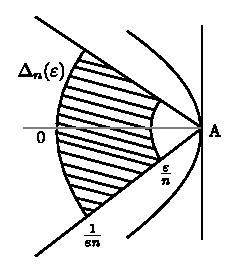
\includegraphics{hayman_fig3.eps}
\end{figure}

\begin{lem}\label{part3-lem4}
We have as $n\to \infty$ uniformly for $z\in\Delta_{n}(\epsilon)$,
$f(z)\sim f_{n}(z)$ and $f'(z)\sim f'_{n}(z)$.
\end{lem}

\begin{proof}
Put $z=l_{n}(w)=r_{n}+\dfrac{1}{n}w$, so that
$(1-z)=\dfrac{1}{n}(1-w)$.

Then by this $\Delta_{n}(\epsilon)$ in the $z$-plane corresponds to
$\Delta_{1}(\epsilon)$ in the $w$ plane. Define a function $g_{n}(z)$
as
$$
g_{n}(w)=(1-w)^{2}\frac{f[l_{n}(w)]}{f(r_{n})}
$$
Note that for a fixed $\epsilon$, $\Delta_{n}(\epsilon)$ lies in
$|z|<1$ for large $n$. Hence $g_{n}(w)$ is defined in
$\Delta_{1}(\epsilon)$ for sufficiently large $n$.
\end{proof}

Further $|g_{n}(w)|=O(1)$ for $w\in\Delta_{1}(\epsilon)$ and
$n>n_{0}$. In fact if $\Delta_{n}(\epsilon)$,
$\Delta_{n}(\frac{1}{2}\epsilon)$, $\Delta_{n}(\frac{1}{4}\epsilon)$
are denoted by $\Delta_{n}$, $\Delta'_{n}$ and $\ub{d}$ 
is\pageoriginale the distance from $\Delta'_{1}$ to the outside of
$\Delta''_{1}$, the distance between $\Delta'_{n}$ and the exterior of
$\Delta''_{n}$ is exactly $d/n$.

So if $\Delta''_{n}$ lies in $|z|<1$. $\Delta'_{n}$ lies in
$|z|<1-\dfrac{d}{n}$ and $\Delta''_{n}$ lies in $|z|<1$ for all large
$n$. Now $|f(z)|\leq \dfrac{r}{(1-r)^{2}}$; $|z|=r$ and so if
$|z|<1-\dfrac{d}{n}<1$; $1-|z|\geq \dfrac{d}{n}$.

Hence in
$\Delta'_{n}|f(z)|=O\left(\dfrac{n^{2}}{d^{2}}\right)=O(n^{2})$ as
$n\to \infty$ and $f(r_{n})=f\left(1-\dfrac{1}{n}\right)\sim \alpha
n^{2}$ by theorem \ref{part3-thm11} as $n\to \infty$ and hence it
follows that
$\dfrac{f[l_{n}(w)]}{f(r_{n})}=\dfrac{O(n^{2})}{n^{2}}=O(1)$ as
$n\to \infty$ uniformly for $w$ in $\Delta'_{1}$. \iec $g_{n}(w)$ is
bounded in $\Delta'_{1}$ for large $n$.

Next choose $-1<w<0$ so that $w$ is real and
$r_{n}+\dfrac{1}{n}w=1-\dfrac{1}{n}(1-w)=l_{n}(w)$. After theorem
\ref{part3-thm12}.
$$
\frac{f[l_{n}(w)]}{f(r_{n})}\sim
\frac{(1-r_{n})^{2}}{\frac{1}{n^{2}}(1-w)^{2}}=\frac{1}{(1-w)^{2}}\quad\text{as}\quad
n\to \infty
$$
for the hypothesis of theorem \ref{part3-thm12} is satisfied because, 
$$
|z|=\left|1-\frac{1}{n}+\frac{1}{n}w\right|<r_{n}<\frac{1}{2}|(z+1)|,
r_{n}\to 1\quad\text{as}\quad n\to \infty
$$
in this manner ensuring the above asymptotic equality.

Therefore it follows on bringing $(1-w)^{2}$ to the left hand side
$g_{n}(w)=(1-w)^{2}\dfrac{f[l_{n}(w)]}{f(r_{n})}$ tends to one as
$n\to \infty$, for real $w$ satisfying $0>w>-1$.

Thus\pageoriginale we have obtained $g_{n}(w)=O(1)$ as $w$ ranges in
$\Delta'_{1}$ and $g_{n}(w)\to 1$ as $n\to \infty$ on a set of $w$
having a limit in $\Delta'_{1}$. Hence by Vitalis convergence theorem
(see Titchmarsh p.p.\@ 168) $g_{n}(w)\to 1$, $g'_{n}(w)\to 0$
uniformly in $\Delta_{1}$ which is contained in $\Delta'_{1}$ and
satisfies the condition that it is bounded by a contour that is
interior to $\Delta'_{1}$.

Now translating back into $z$, $n^{2}(1-z)^{2}\dfrac{f(z)}{f(r_{n})}$
tends to $1$ as $n$ tends to infinity for $z\in \Delta_{n}(\epsilon)$.

\ie by the definition of $f_{n}(z)$
$$
\frac{f(z)}{f_{n}(z)}\to 1\quad\text{for}\quad z\in
\Delta_{n}(\epsilon)\quad\text{as}\quad n\to \infty.
$$
Also
$$
\frac{d}{dw}(1-w)^{2}\frac{f[l_{n}(w)]}{f(r_{n})}\to 0
$$
since $n(1-z)=(1-w)$;
$\frac{1}{n}\dfrac{d}{dz}n^{2}(1-z)^{2}\dfrac{f(z)}{f(r_{n})}\to 0$
\begin{align*}
& n\frac{d}{dz}(1-z)^{2}\frac{f(z)}{f(r_{n})}\to 0\\
& \frac{d}{dz}(1-z)^{2}f(z)= O(n)\text{ \  since \ }
  f(r_{n})\sim\alpha n^{2}\text{ \ as \ } n\to \infty.
\end{align*}
for $z$ in $\Delta_{n}(\epsilon)$.

Note that in $\Delta_{n}(\epsilon)\dfrac{1}{n}$ and $(1-z)$ have the
same order of magnitude.

Thus,\pageoriginale $(1-z)^{2}f'(z)-2(1-z)f(z)=0(n)$, $z\in
\Delta_{n}(\epsilon)$ as $n\to \infty$
\begin{align*}
f'(z) &= \frac{2f(z)}{(1-z)}+O(n^{3}), \;\; z\in\Delta_{n}(\epsilon)\text{
  \  as \ } n\to \infty.\\
&= \frac{2f_{n}(z)}{(1-z)}+O(n^{3})\\
&= f'_{n}(z)+O(n^{3})=f'_{n}(z)[1+O(1)]
\end{align*}
because
$$
f'_{n}(z)=\frac{2\alpha n}{(1-z)}=O(n^{3}).
$$

Therefore, $f'(z)\sim f'_{n}(z)$ uniformly for
$z\in\Delta_{n}(\epsilon)$ as $n\to \infty$. This completes the proof
of the lemma.

\begin{lem}\label{part3-lem5}
With the notation of theorem \ref{part3-thm4}, for $\lambda>0$,
$$
S_{\lambda}(r,f)=\alpha^{\lambda}S_{\lambda}[r,(1-z)^{-2}] +
O(1-r)^{-2\lambda}\text{ 
  \  as \ }r\to 1
$$
and if $\lambda>\dfrac{1}{2}$
$$
I_{\lambda}(r,f)=\alpha^{\lambda}I_{\lambda}[r,(1-z)^{-2}] + O
(1-r)^{1-2\lambda}\text{  \ as \ } r\to 1
$$
\end{lem}

\begin{proof}
Let $R_{n}=|\alpha_{n}|\dfrac{n^{2}}{\epsilon^{2}}$,
$\varphi_{n}(z)=f_{n}(z)^{\lambda}=\alpha^{\lambda}_{n}(1-z)^{-2\lambda}$
and $\Delta_{n}(\epsilon)$ as defined in the\pageoriginale previous
lemma. Note that $\varphi_{n}(z)$ maps $\Delta_{n}(\epsilon)$ onto the
sector
$$
\epsilon^{4\lambda}R^{\lambda}_{n}<|w|<R^{\lambda}_{n},
|\arg(w)-\lambda\arg\alpha_{n}|<(\pi -2\epsilon)
$$
The area of the image \; $=\iint\limits_{\Delta_{n}(\epsilon)}
|\varphi'_{n}(z)|^{2}\ dx\ dy $
\begin{equation*}
=\lambda(\pi-2\epsilon)R^{2\lambda}_{n} [1-\epsilon^{8\lambda}]
\tag{3.2.1}\label{part3-eq3.2.1}  
\end{equation*}
Also in $\Delta_{n}(\epsilon)$, $f_{n}(z)\sim f(z)$ and $f'_{n}(z)\sim
f'(z)$ and so
$$
\varphi'_{n}(z)=\lambda f'_{n}(z)[f_{n}(z)]^{\lambda-1}\sim \lambda
f'(z)[f(z)]^{\lambda-1}=\varphi'(z) 
$$
So we have 
\begin{equation*}
\iint\limits_{\Delta_{n}(\epsilon)} |\phi'_n(z)|^{2}dx\ dy\sim
\lambda(\pi-2\epsilon)R^{2\lambda}_{n}(1-\epsilon^{8\lambda})\tag{3.2.2}\label{part3-eq3.2.2} 
\end{equation*}
Also since $|\varphi_{n}(z)|<R^{\lambda}_{n}$ in
$\Delta_{n}(\epsilon)$ we have by lemma \ref{part3-lem4},
$$
|\varphi(z)|<R^{\lambda}_{n}(1+\epsilon)\quad\text{there for large \ } n.
$$
Now choose $n$ so that $R_{n-1}<M(r,f)<R_{n}$. This is possible at
least if $r$ is sufficiently near $1$, since $R_{n}\to \infty$ with $n$.
\end{proof}

Let $E_{0}$ be the set of points of $|z|<r$ outside
$\Delta_{n}(\epsilon)$. Then in $E_{0}$,
$|\varphi(z)|<R^{\lambda}_{n}$, and in $\Delta_{n}(\epsilon)$,
$|\varphi(z)|<(1+\epsilon)R^{\lambda}_{n}$. The image of $|z|<1$ by
$f(z)$ contains no point more than once, and so the length of the
image over any circle $|w|=\rho$ is at the most $2\pi\rho$.

If we cut the unit circle along the negative real axis, then the image
by $f(z)^{\lambda}$ covers any circle, $|w|=\rho$, with length at the
most $\lambda 2\pi\rho$. So the area of the image of the union of
$E_{0}$ and $\Delta_{n}(\epsilon)$ by $\varphi(z)$ is at most $\pi
\lambda R^{2\lambda}_{n}(1+\epsilon)^{2}$.

That\pageoriginale gives,
$$
\iint\limits_{E_{0}\cup
  \Delta_{n}(\epsilon)}|\varphi'(z)|^{2}dx\ dy\leq \pi\lambda
  R^{2\lambda}_{n}(1+\epsilon)^{2} 
$$
Also by \eqref{part3-eq3.2.2}, we have for large $n$
$$
\iint\limits_{\Delta_{n}(\epsilon)}|\varphi'(z)|^{2}dx\ dy>\lambda\pi
(1-\epsilon)(1-\epsilon^{8\lambda})R^{2\lambda}_{n}
$$
[Note the $\epsilon$ terms of r.h.s.\@ of this inequality and
  \eqref{part3-eq3.2.2}] 

So
\begin{gather*}
\iint\limits_{E_{0}}|\varphi'(z)|^{2}dx\ dy<R^{2\lambda}_{n}\pi\lambda\left[(1+\epsilon)^{2}-(1-\epsilon)(1-\epsilon^{8\lambda})\right]\\
<\epsilon^{1}R^{2\lambda}_{n}
\end{gather*}
where $\epsilon^{1}$ is small if $\epsilon$ is small.

Similarly,
$$
\iint\limits_{E_{0}}|\varphi'_{n}(z)|^{2}dx\ dy<\epsilon''R^{2\lambda}_{n}
$$
By theorem \ref{part3-thm4}
\begin{align*}
S_{2\lambda}(r,f) &= \frac{\lambda^{2}}{2\pi}\int\limits^{r}_{0}\rho
d\rho \int\limits^{\pi}_{-\pi}|f(\rho
e^{i\theta})|^{2\lambda-2}|f'(\rho e^{i\theta})|^{2}d\theta\\
&= \frac{\lambda^{2}}{2\pi}\iint\limits_{|z|<r}|f(\rho
e^{i\theta})|^{2\lambda-2}|f'(\rho e^{i\theta})|^{2}dx\ dy\\
&= \frac{1}{2\pi}\iint\limits_{|z|<r}|\varphi'(z)|^{2}dx\ dy.
\end{align*}\pageoriginale
Hence
\begin{align*}
S_{2\lambda}(r,f)-S_{2\lambda}(r,f_{n}) &=
\frac{2}{\pi}\iint\limits_{|z|<r}
\left(|\varphi'(z)|^{2}-|\varphi'_{n}(z)|^{2} \right) \ dx\ dy\\
&= \frac{2}{\pi}\left[\int\limits_{E_{1}}+\int\limits_{E_{0}}\right]
\end{align*}
where $E_{1}$ is the part of $|z|<r$ within
$\Delta_{n}(\epsilon)$. Since in $E_{1}\varphi'_{n}(z)\sim
\varphi'(z)$ 
\begin{align*}
\int\limits_{E_{1}}
\left(|\varphi'(z)|^{2}-|\varphi'_{n}(z)|^{2}\right) \ dx\ dy &=
O\int\limits_{E_{1}}|\varphi'_{n}(z)|^{2}dx\ dy\\
&= O\int\limits_{\Delta_{n}(\epsilon)}|\varphi'_{n}(z)|^{2}dx\ dy\\
&= O(R^{2}_{n})\quad\text{by \eqref{part3-eq3.2.1}}
\end{align*}
Also
\begin{align*}
|\int\limits_{E_{0}}\left(|\varphi'(z)|^{2}-|\varphi'_{n}(z)|^{2}
\right) \ dx\ dy | &\leq
\int\limits_{E_{0}}|\varphi'_{n}(z)|^{2} \ dx\ dy +
\int\limits_{E_{0}}|\varphi'(z)|^{2} \ dx\ dy\\ 
&\leq (\epsilon''+\epsilon')R^{2}_{n}.
\end{align*}
Since $\epsilon''$ and $\epsilon'$ can be made as small as we please
by suitable choice of $\epsilon$,
\begin{align*}
S_{2\lambda}(r,f) &=S_{2\lambda}(r,f_{n}) + O(R^{2\lambda}_{n})\\
&= S_{2\lambda}(r,f_{n})+ O(R^{2\lambda}_{n-1})\quad\text{as}\quad R_{n}\sim
R_{n-1}\\
&= S_{2\lambda}(r,f_{n}) + OM(r,f)^{2\lambda}.
\end{align*}\pageoriginale
\ie $S_{2\lambda}(r,f)=S_{2\lambda}(r,f_{n})+O(1-r)^{-4\lambda}$ as
$r\to 1$ (by theorem \ref{part3-thm3}).

Hence we get
$$
S_{2\lambda}(r,f)=|\alpha^{2\lambda}_{n}|S_{2\lambda}[r,(1-z)^{-2}] +
O(1-r)^{-4\lambda}\quad\text{as}\quad 
r\to 1.
$$
which is the first result. Integrating the above from $0$ to $r$,
w.r.t.\@ $r$ after dividing by $r$, we get
$$
I_{2\lambda}(r,f)=|\alpha|^{2\lambda}I_{\lambda}[r,(1-z)^{-2}] +
O(1-r)^{1-4\lambda}\text{   \  as \ } r\to 1, \text{ \  if \ }
\lambda>\frac{1}{4}. 
$$
Hence we get the lemma [replacing $2\lambda$ by $\lambda$]
$$
I_{\lambda}(r,f)=\alpha^{\lambda}I_{\lambda}
[r,(1-z)^{-2}] + O(1-r)^{1-2\lambda}\text{ \ as \ } r\to 1 
$$
if $\lambda>\dfrac{1}{2}$.

\begin{lem}\label{part3-lem6}
If \, $\eta>0$ \, and \, $\lambda>\dfrac{1}{4}$ \, we can choose \,
$k>0$ \, so that if \; $r_{0}<r<1$, $1-\dfrac{1}{n}\leq r\leq 1-\dfrac{1}{2n}$ 
$$
\int\limits_{k(1-r)\leq |\theta|\leq
  \pi} \left( |f(re^{i\theta})|^{2}+|f_{n}(re^{i\theta})|^{2} \right)
d\theta<\eta(1-r)^{1-4\lambda}  
$$
\end{lem}

Let $\gamma$ and $\gamma \,'$ be the arcs $|\theta|\leq k(1-r)$ and
$k(1-r)\leq |\theta|\leq \pi$ on $|z|=r$. If $k$ is any fixed number,
we can choose $\epsilon$ so small that the\pageoriginale arc $\gamma$
lies in $\Delta_{n}(\varepsilon)$ for $1-\dfrac{1}{n}\leq r\leq
1-\dfrac{1}{2n}$ for large $n$ (see Hayman \cite{1}).

Hence
$$
\int\limits_{\gamma}|f_{n}(z)|^{2\lambda}d\theta\sim \int\limits_{\gamma}|f(z)|^{2\lambda}d\theta
$$
\begin{align*}
\int\limits_{\gamma}|f_{n}|^{2\lambda}d\theta-\int\limits_{\gamma}|f|^{2\lambda}
d\theta &= O\int|f|^{2\lambda}d\theta\\
&= O\{I_{2\lambda}(r,f)\}\\
&= O(1-r)^{1-4\lambda}
\end{align*}
by the application of theorem \ref{part3-thm4}, as
$2\lambda>\dfrac{1}{2}$ and also
$I_{2\lambda}(r,f)-I_{2\lambda}(r,f_{n})=O[(1-r)^{1-4\lambda}]$ by the
previous lemma.

Hence subtraction gives,
\begin{equation*}
\int\limits_{\gamma\,'}|f|^{2\lambda}d\theta
-\int\limits_{\gamma\,'}|f_{n}|^{2\lambda}d\theta
=O[(1-r)^{1-4\lambda}]\tag{3.2.3}\label{part3-eq3.2.3} 
\end{equation*}
Now the integral
\begin{gather*}
\int\limits_{\gamma \,'}|f_{n}|^{2\lambda}d\theta
\int\limits^{\pi}_{k(1-r)}\frac{|\alpha_{n}|^{2\lambda}d\theta}{(1-2r\cos
  \theta+r^{2})^{2 \lambda}}\\
\leq \int\limits^{\pi}_{k(1-r)}\frac{d\theta}{(r\sin
  \theta/2)^{4\lambda}}\\
A(\lambda)\int\limits^{\infty}_{k(1-r)}\frac{d\theta}{\theta^{4\lambda}}
\end{gather*}
$\dfrac{1}{(1-2r\cos\theta+r^{2})}\leq
\dfrac{1}{(r\sin^{2}\theta/2)^{2}}\sin\theta/2\geq A\theta$ in that
range.
\begin{align*}
\int\limits_{\gamma \,'}|f_{n}|^{2\lambda}d\theta & \leq
A(\lambda)[k(1-r)]^{1-4\lambda}\tag{4}\label{part3-eq4}\\ 
&< \frac{1}{3}\eta (1-r)^{1-4\lambda}
\end{align*}\pageoriginale
by properly choosing $k$ sufficiently large. Hence in virtue of the
relation \eqref{part3-eq2} we deduce same for $f(z)$ and hence the
lemma. 

We now proceed to prove theorem \ref{part3-thm13}. We have as in lemma
\ref{part3-lem5}, 
\begin{align*}
\varphi_{n}(z) &=
f_{n}(z)^{\lambda}=\alpha^{\lambda}_{n}(1-z)^{-2\lambda}=\alpha^{\lambda}_{n}\sum^{\infty}_{0}b_{m}z^{m}\\
b_{m} &= \frac{2\lambda(2\lambda+1)\ldots\ldots (2\lambda+m-1)}{m!}\\
&= \frac{\Gamma(m+1+2\lambda)}{\Gamma(2\lambda)\Gamma(m+1)}\sim
\frac{m^{2\lambda-1}}{\Gamma(2\lambda)} 
\end{align*}
and as already defined
$$
\varphi(z)=z^{\lambda}\left[1+\sum^{\infty}_{m=1}a_{m,\lambda}z^{m}\right]
$$
Hence by considering the coefficients of $\varphi'(z)$ and
$\varphi'_{n}(z)$,
\begin{gather*}
(n+\lambda)a_{n,\lambda}-nb_{n}\alpha^{\lambda}_{n}=\frac{1}{2\Pi}\int\limits_{|z|=r}\frac{\varphi'(z)}{z^{n+\lambda}}-\frac{\varphi'_{n}(z)}{z^{n}}dz\\
\Big| (n+\lambda)a_{n,\lambda}-nb_{n}\alpha^{\lambda}_{n}\left|\leq
\frac{1}{2\pi}\frac{1}{r^{n+\lambda-1}}\right| \int\limits^{2\pi}_{0}
\left(\varphi'(re^{i\theta})-re^{\lambda
  i\lambda\theta}\varphi'_{n}(re^{i\theta})\right)d\theta 
\end{gather*}
We shall choose $r$ in the range $1-\dfrac{1}{n}\leq r\leq
1-\dfrac{1}{2n}$ as usual. For a $k$ to be determined, let $\gamma$
and $\gamma\,'$ be the arcs $|\theta|\leq k(1-r)$ and $k(1-r)\leq
|\theta|\leq \pi$ respectively on $|z|=r$.
$$
\gamma,\varphi'\sim \varphi'_{n}\circ
(\varphi'_{n})(r^{\lambda}e^{i\lambda\theta})= O(1-r)^{-1-2\lambda}\text{
  \ as \ } r\to 1.
$$\pageoriginale
and so
$$
\varphi'-(\varphi'_{n})(r^{\lambda}e^{i\lambda\theta})=O(1-r)^{-1-2\lambda}
=O(n^{2\lambda+1})\text{
  \ as \ } r\to 1 \text{ \ or as \ } n\to \infty
$$

The length of the path of integration of
$\gamma=O(1-r)=O\left(\dfrac{1}{n}\right)$
$$
\int\left(\varphi'(re^{i\theta})-r^{\lambda}e^{i\lambda\theta}\varphi'_{n}
(re^{i\theta}) \right) d\theta=O(n^{2\lambda}) 
$$
this being true for any fixed $k$.

Again,
\begin{gather*}
|\int\limits_{\gamma \, '}
\left(\varphi'(re^{i\theta}) -
r^{\lambda}e^{i\lambda\theta}\varphi'_{n}(re^{i\theta}) \right)d\theta|\\
\leq \int\limits_{\gamma
  \,'}|\varphi'(re^{i\theta})|d\theta+\int\limits_{\gamma\, '}r^{\lambda}|\varphi'_{n}(re^{i\theta})|d\theta
\end{gather*}
We now proceed as in theorem \ref{part3-thm6}, choose $t$ such that
$2\lambda-2t>\dfrac{1}{2}$ and using Schwarz's Inequality.
\begin{gather*}
\int\limits_{\gamma\, '}|\varphi'(re^{i\theta})|d\theta =
\lambda\int\limits_{\gamma \, '} |f'(re^{i\theta})|
|f(re^{i\theta})|^{\lambda-1}d\theta\\  
\leq \lambda
\left[\int\limits_{\gamma}|f'(re^{i\theta})|^{2}|f(re^{i\theta})|^{2t-2\lambda}d\theta\right]^{\frac{1}{2}}\\
\left[\int\limits_{\gamma \, '}|f(re^{i\theta})|^{2\lambda-2t}d\theta\right]^{\frac{1}{2}} 
\end{gather*}
By the same method as of theorem \ref{part3-thm6}, we can choose $r$
such that the first integral is $O(n^{4t+1})$.

By what we have just seen in lemma \ref{part3-lem6} the second
integral can be made less that $\delta\eta(1-r)^{1-4\lambda+4t}$ \ie
(const.) $\eta n^{4\lambda-4t-1}$ and $\eta$ can be made as small as
we please. So 
$$
\int|\varphi'(re^{i\theta})|d\theta<\eta'n^{2\lambda}
$$\pageoriginale
using the inequality (8) of theorem \ref{part3-thm6}.

$\eta'$ can be made as small as we please by choosing $k$ large enough
$\int\limits_{\gamma \, '}\varphi'_{n}(re^{i\theta})d\theta$ can be
dealt with similarly.

So finally we see that
$$
\int\limits^{2\pi}_{0}| [\varphi'(re^{i\theta}) - r^{\lambda}
e^{i\lambda\theta} \varphi \,'_{n}(re^{i\theta})]d\theta\leq
[2\eta\, ' + O (1)]n^{2\lambda}
$$
and since $\eta'$ can be made as small as we please the right hand
side is $O(n^{2\lambda})$.

That gives 
\begin{align*}
a_{n,\lambda} &=
\frac{nb_{n}\alpha^{\lambda}_{n}}{n+\lambda} + O(n^{2\lambda-1})\\
&=
\frac{n}{n+\lambda}\frac{f(r_{n})^{\lambda}}{n^{2\lambda}}
\frac{n^{2\lambda-1}}{\Gamma(2\lambda)}+O(n^{2\lambda-1}) 
\end{align*}
Therefore,
$$
na_{n,\lambda}\sim \dfrac{f(r_{n})^{\lambda}}{\Gamma(2\lambda)}\text{
  \ as required.}
$$

This completes the proof of theorem \ref{part3-thm13}. For an
extension of the result to $p$-valent functions and further results
see for example W.K.\@ Hayman \cite{1}, \cite{2}.

\begin{thebibliography}{99}\pageoriginale
\bibitem{1} Ahlfors, L.\@ \cite{1}:~ Beitrage Zur Theorie der
  meromorphen Funktionen 7, Congr.\@ Math.\@ Scand.\@ Oslo 1929.

\bibitem{2} Bazilevi\v{c}, I.E.\@ \cite{1}:~ On distortion theorem and
  coefficients of univalent functions. Mat.\@ Sbornik N.S.\@ 28 (70),
  283-292 (1951).

\bibitem{3} Biernacki, M.\@ \cite{1}:~ Bull.\@ Acad.\@ Polon.\@ Sci.\@
  Cl.III 4 (1956) 5-8

\bibitem{4} Carath\'eodory, C.\@ \cite{2}:~ ``Theory of Functions of
  one variable'' Vol.I Translated by Steinhardt

\bibitem{5} Csillag, P.\@ \cite{1}:~ Math.\@ Annalen 110 (1935) pp.\@
  745-'52.

\bibitem{6} Hayman, W.K.\@ \cite{1}:~ Proc.\@ L.M.S.\@ 1955 p.p.\@
  257-284.

\bibitem{7} Hayman, W.K.\@ \cite{2}:~ ``Multivalent Functions''
  Cambridge University Press.

\bibitem{8} Hayman, W.K.\@ and Stewart, F.M.\@ \cite{1}:~ Proc.\@
  Camb.\@ Phil.\@ Soc.\@ 1954.

\bibitem{9} Kaplan, W.\@ \cite{1}:~ (`close to convex Schlicht
  functions') Michigan Math.\@ J.\@ 1(1953) 169-'85.

\bibitem{10} Kennedy, P.B.\@ \cite{1}:~ Proc.\@ L.M.S.\@ Vol.\@ 6
  1956.

\bibitem{11} Little wood, D.\@ \cite{1}:~ Q.J.\@ of Maths.\@ Vol.9
  (1938)

\bibitem{12} Shimizu, T.\@ \cite{1}:~ On the Theory of Meromorphic
  Functions Jap.\@ J.\@ Maths.\@ 6 (1929).
\end{thebibliography}







